\chapter{Réalisation et Présentation des Interfaces}
\label{chap:realisation}

\section{Introduction}

Ce chapitre présente la concrétisation pratique de la plateforme logicielle \textbf{PMS AMH Hospitality}. Nous débuterons par la description détaillée de l'architecture technique microservices déployée sous conteneurs Docker, puis nous exposerons de manière exhaustive l'ensemble des interfaces utilisateurs développées, accompagnées de leurs captures d'écran réelles issues des phases d'essais en situation opérationnelle et d'explications fonctionnelles et techniques approfondies. Nous achèverons ce chapitre par le bilan des contributions individuelles de chaque élève-ingénieur et la synthèse des défis techniques surmontés.

\section{Architecture technique globale des microservices}

La Figure~\ref{fig:arch_technique} expose la cartographie complète de l'architecture microservices déployée au sein de l'infrastructure d'AMH Hospitality.

\begin{figure}[H]
\centering
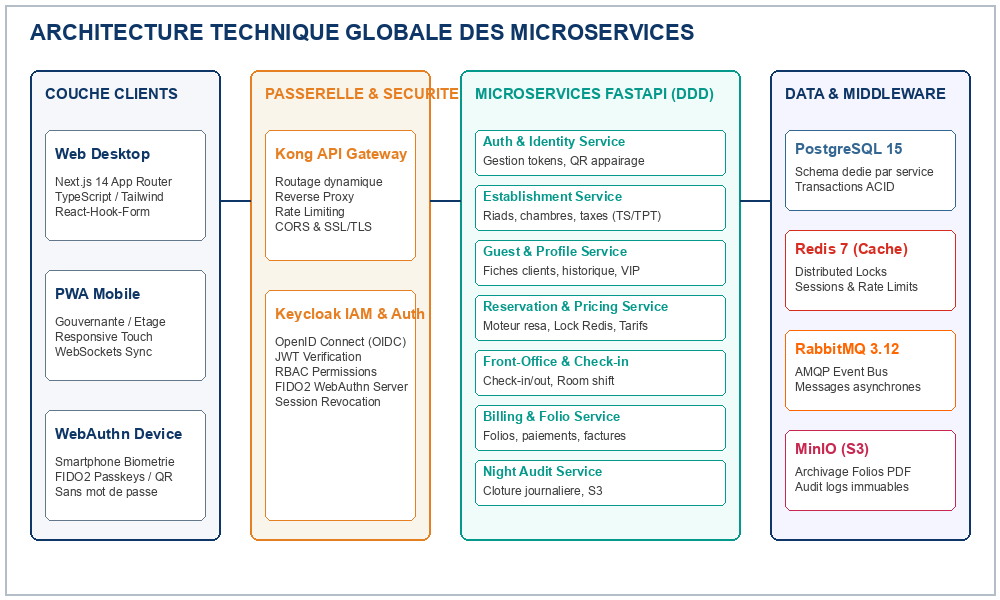
\includegraphics[width=0.95\textwidth]{figures/arch_technique.png}
\caption{Architecture technique globale des microservices PMS AMH Hospitality}
\label{fig:arch_technique}
\end{figure}

Comme l'illustre la Figure~\ref{fig:arch_technique}, l'architecture s'articule autour de quatre couches interdépendantes :
\begin{enumerate}
    \item \textbf{Couche Clients et Présentation} : 
    \begin{itemize}
        \item Application Web Desktop développée sous Next.js 14 (React 18, TypeScript, Tailwind CSS) pour les postes de réception et les postes administratifs ;
        \item Progressive Web App (PWA) mobile réactive optimisée pour les smartphones des gouvernantes et du personnel d'étage ;
        \item Terminal biométrique mobile (smartphone de l'utilisateur) pour la signature des challenges d'authentification WebAuthn/FIDO2.
    \end{itemize}
    \item \textbf{Couche Passerelle d'API et Sécurité Périmétrique} :
    \begin{itemize}
        \item \textit{Kong API Gateway} : Point d'entrée unique assurant le routage dynamique des requêtes HTTP, le filtrage CORS, l'équilibrage de charge, la terminaison SSL/TLS et la limitation de débit (\textit{Rate Limiting}) ;
        \item \textit{Keycloak IAM} : Serveur d'authentification centralisé gérant les utilisateurs, les jetons JWT OIDC signés asymétriquement (RS256) et l'enregistrement des clés publiques FIDO2.
    \end{itemize}
    \item \textbf{Couche Cœur Métier (Microservices FastAPI)} : Onze services autonomes et spécialisés fonctionnant dans des conteneurs isolés :
    \begin{itemize}
        \item \texttt{Auth \& Identity Service} : Gestion des sessions et flux Passkey QR ;
        \item \texttt{Establishment Service} : Référentiel des Riads, chambres, équipements et Business Date ;
        \item \texttt{Guest Profile Service} : Répertoire des voyageurs et segmentation VIP ;
        \item \texttt{Reservation Service} : Moteur de réservation, tarification et verrous Redis ;
        \item \texttt{Front-Office Service} : Gestion du Check-in/out et réattribution de chambres ;
        \item \texttt{Billing \& Folio Service} : Comptes folios, calcul fiscal (TVA, TS, TPT) et factures PDF ;
        \item \texttt{Night Audit Service} : Moteur de clôture nocturne transactionnelle et archivage ;
        \item \texttt{Housekeeping Service} : Suivi du nettoyage d'étage et diffusion WebSocket ;
        \item \texttt{Notification Service} : Routage des alertes événementielles temps réel ;
        \item \texttt{Channel Manager Service} : Passerelle de synchronisation avec les plateformes OTA ;
        \item \texttt{Reporting Service} : Calcul des KPI consolidés (RevPAR, ADR, taux d'occupation).
    \end{itemize}
    \item \textbf{Couche Données et Intergiciels} :
    \begin{itemize}
        \item Instances PostgreSQL 15 dédiées avec schémas étanches par microservice ;
        \item Instance Redis 7 assurant le cache haute vitesse et les verrous distribués à bail TTL ;
        \item Courtier RabbitMQ 3.12 assurant la persistance des messages AMQP sur files durables ;
        \item Stockage objet MinIO S3 archivant de manière immuable les rapports de clôture et factures.
    \end{itemize}
\end{enumerate}

\section{Présentation détaillée des interfaces utilisateurs}

\subsection{Module 1 : Authentification et gestion des accès}

\subsubsection{Interface d'authentification sans mot de passe WebAuthn / Passkey}

La Figure~\ref{fig:passkey} présente l'interface principale de connexion à la plateforme.

\begin{figure}[H]
\centering
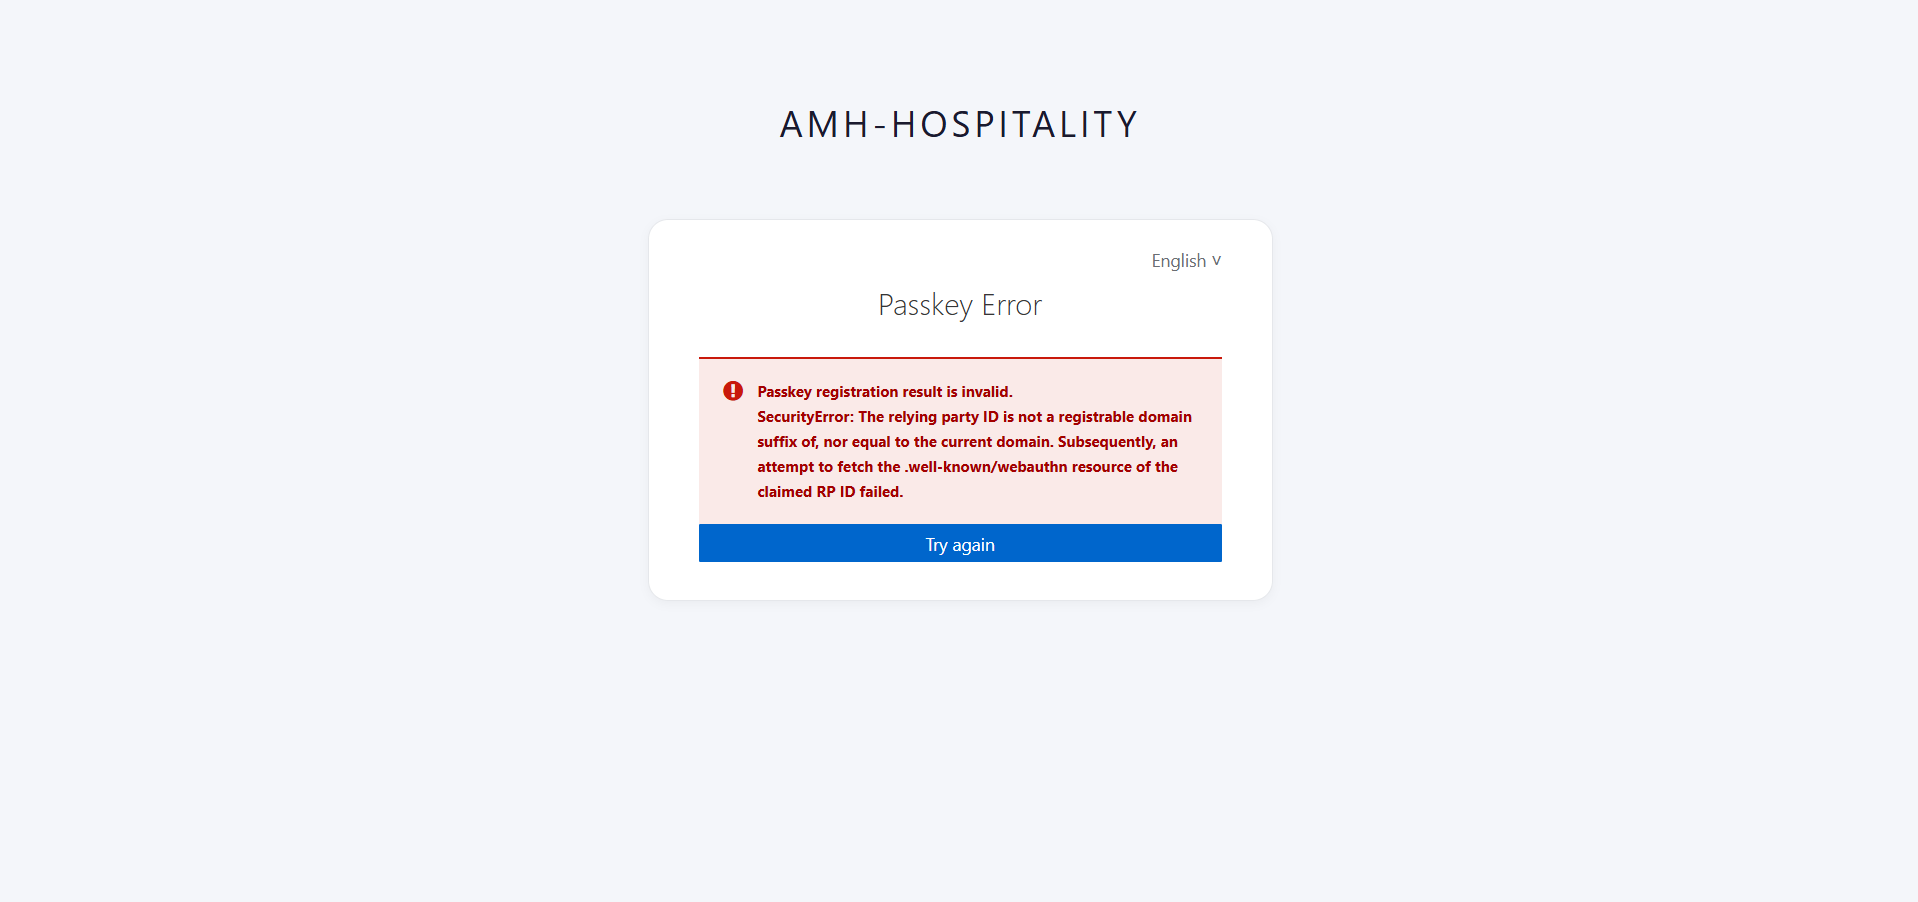
\includegraphics[width=0.85\textwidth]{figures/passkey.png}
\caption{Interface d'authentification sans mot de passe WebAuthn / Passkey}
\label{fig:passkey}
\end{figure}

L'interface présentée dans la Figure~\ref{fig:passkey} offre un double mécanisme d'authentification : la méthode classique par identifiant et mot de passe chiffré, et la méthode moderne par clé d'accès biométrique (\textit{Passkey}). L'utilisateur peut enregistrer son terminal mobile en un clic ; lors des connexions ultérieures, un simple clic sur « Se connecter avec Passkey » déclenche la vérification biométrique en moins de 2 secondes, éliminant tout risque de piratage par force brute ou vol d'identifiants.

\subsubsection{Interface d'appairage mobile par QR Code dynamique}

La Figure~\ref{fig:pms_link_qr} illustre l'interface d'appairage par QR Code sur poste fixe de réception.

\begin{figure}[H]
\centering

\includegraphics[width=0.4\textwidth]{figures/pms_link_qr.png}
\caption{Interface d'appairage mobile par QR Code dynamique}
\label{fig:pms_link_qr}
\end{figure}

Comme l'illustre la Figure~\ref{fig:pms_link_qr}, lorsqu'un réceptionniste s'installe sur un poste de travail partagé, le système génère un QR code dynamique contenant un identifiant de session éphémère et un challenge cryptographique. Le réceptionniste scanne ce code avec l'appareil photo de son smartphone, valide son empreinte digitale (TouchID) ou son visage (FaceID), ce qui déverrouille instantanément sa session nominative sur le poste de réception sans qu'aucun mot de passe ne soit saisi sur le clavier partagé.

\subsubsection{Interface de gestion des jetons JWT et des sessions actives}

La Figure~\ref{fig:jeton} présente l'écran d'administration des sessions de sécurité.

\begin{figure}[H]
\centering
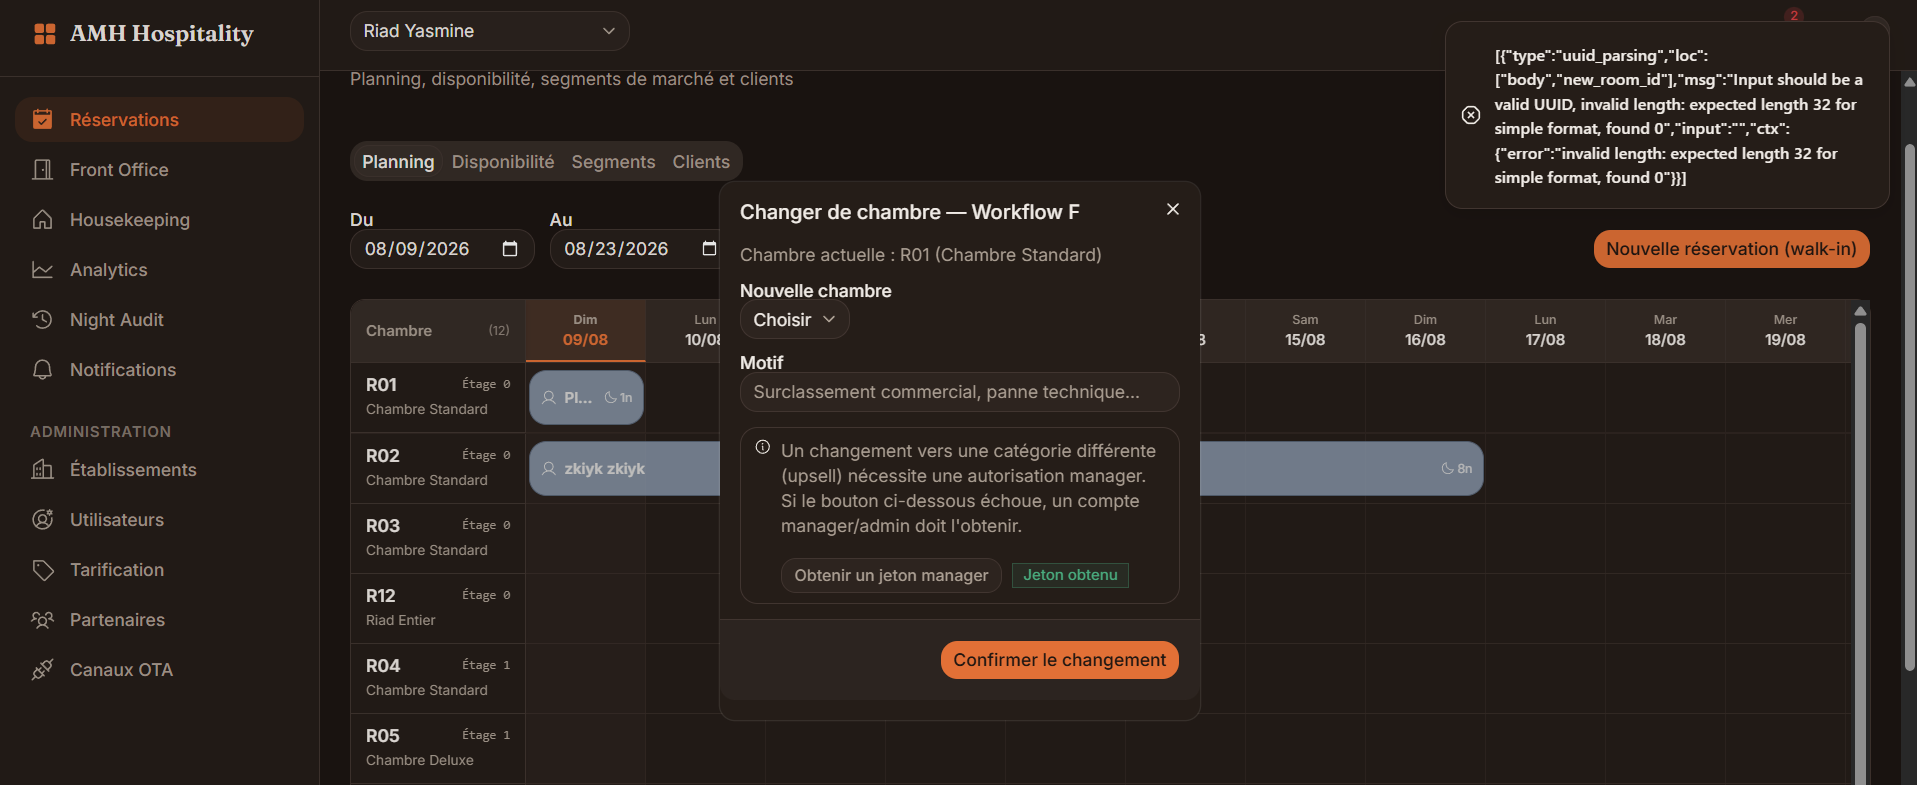
\includegraphics[width=0.85\textwidth]{figures/jeton.png}
\caption{Interface de gestion des jetons d'authentification et sessions actives}
\label{fig:jeton}
\end{figure}

La Figure~\ref{fig:jeton} permet aux administrateurs de visualiser en temps réel l'ensemble des sessions connectées sur la plateforme (adresse IP, terminal, rôle, Riad actif, heure de délivrance du jeton JWT). En cas de suspicion d'activité anormale ou de départ d'un collaborateur, l'administrateur peut révoquer instantanément un jeton via une inscription dans la \textit{blacklist} distribuée sous Redis.

\subsection{Module 2 : Tableau de bord et planification des séjours}

\subsubsection{Interface Tableau de bord principal d'exploitation}

La Figure~\ref{fig:homepage} expose la vue d'ensemble opérationnelle du Riad.

\begin{figure}[H]
\centering
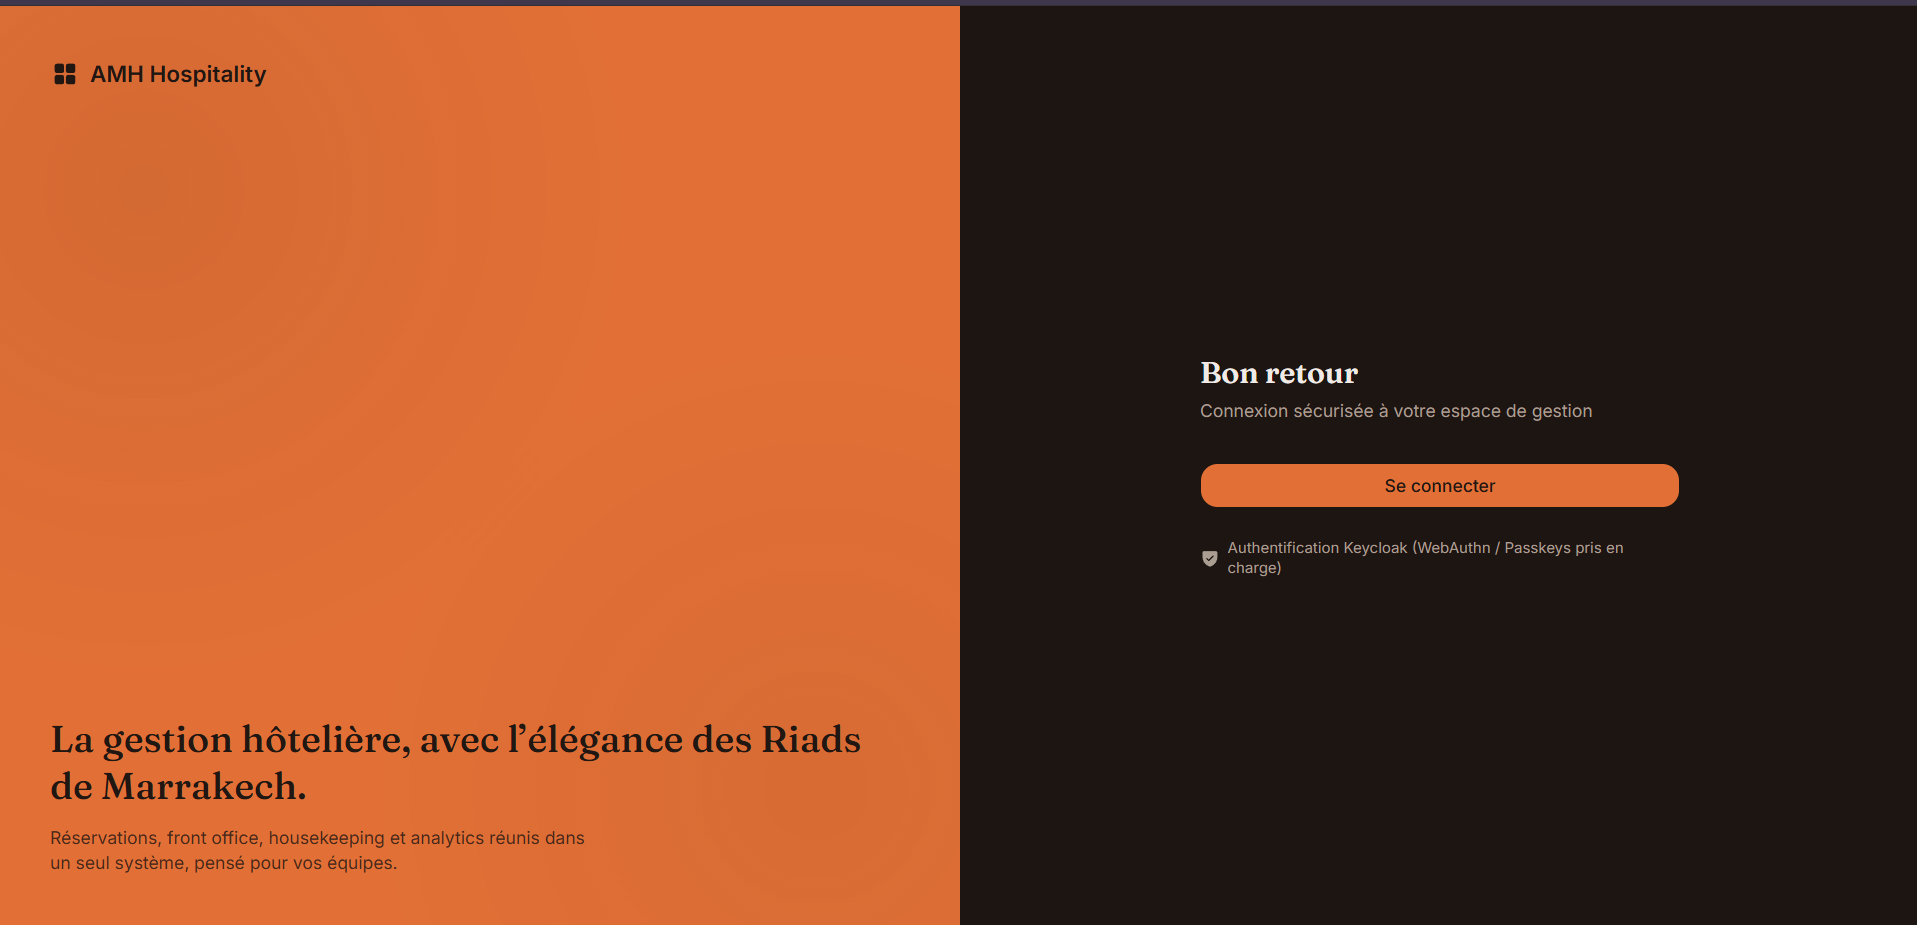
\includegraphics[width=0.9\textwidth]{figures/homepage.png}
\caption{Interface Tableau de bord principal (Vue d'ensemble du Riad)}
\label{fig:homepage}
\end{figure}

Le tableau de bord (Figure~\ref{fig:homepage}) constitue l'écran d'accueil quotidien des réceptionnistes et directeurs de Riad. Il affiche sous forme de cartes d'indicateurs synthétiques :
\begin{itemize}
    \item Le nombre d'arrivées prévues dans la journée avec statut de préparation de la suite ;
    \item Le nombre de départs programmés avec indicateur de solde du folio (vert si soldé, orange si en attente d'encaissement) ;
    \item Le taux d'occupation journalier et le nombre de chambres disponibles ;
    \item L'état global du parc de chambres (propres, en cours de nettoyage, sales, hors service) actualisé en temps réel via WebSockets.
\end{itemize}

\subsubsection{Interface Planning interactif des chambres (Tape Chart matriciel)}

La Figure~\ref{fig:table_} présente le planning matriciel interactif des chambres.

\begin{figure}[H]
\centering
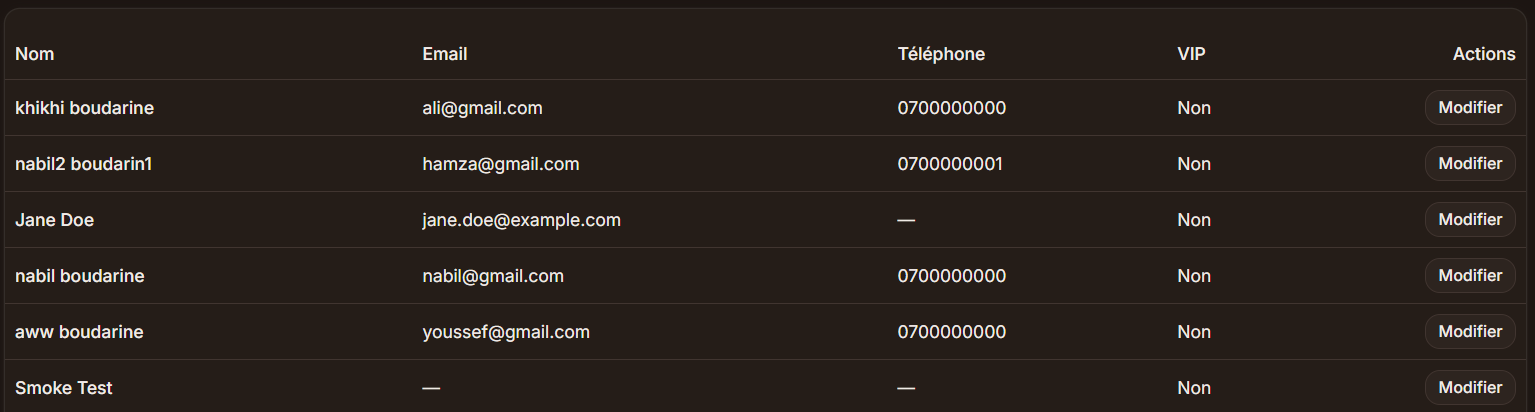
\includegraphics[width=0.95\textwidth]{figures/table_.png}
\caption{Interface Planning interactif des chambres (Tape Chart Drag \& Drop)}
\label{fig:table_}
\end{figure}

Le Tape Chart (Figure~\ref{fig:table_}) est l'outil central de travail en réception. Il présente une grille matricielle où les lignes représentent les chambres physiques (triées par étage et catégorie : Suite Royale, Suite Junior, Chambre Deluxe) et les colonnes représentent l'axe temporel (jours). Les séjours sont visualisés sous forme de blocs horizontaux dont la couleur indique l'état (bleu = confirmé, vert = in-house, gris = checked-out). L'interface supporte la manipulation par glisser-déposer (\textit{Drag \& Drop}) pour changer une réservation de chambre ou prolonger un séjour, avec recalcul automatique instantané des montants financiers.

\subsection{Module 3 : Réservations et gestion des flux d'arrivée/départ}

\subsubsection{Interface de création et modification de réservation}

La Figure~\ref{fig:reservation} expose le formulaire complet de création de réservation.

\begin{figure}[H]
\centering
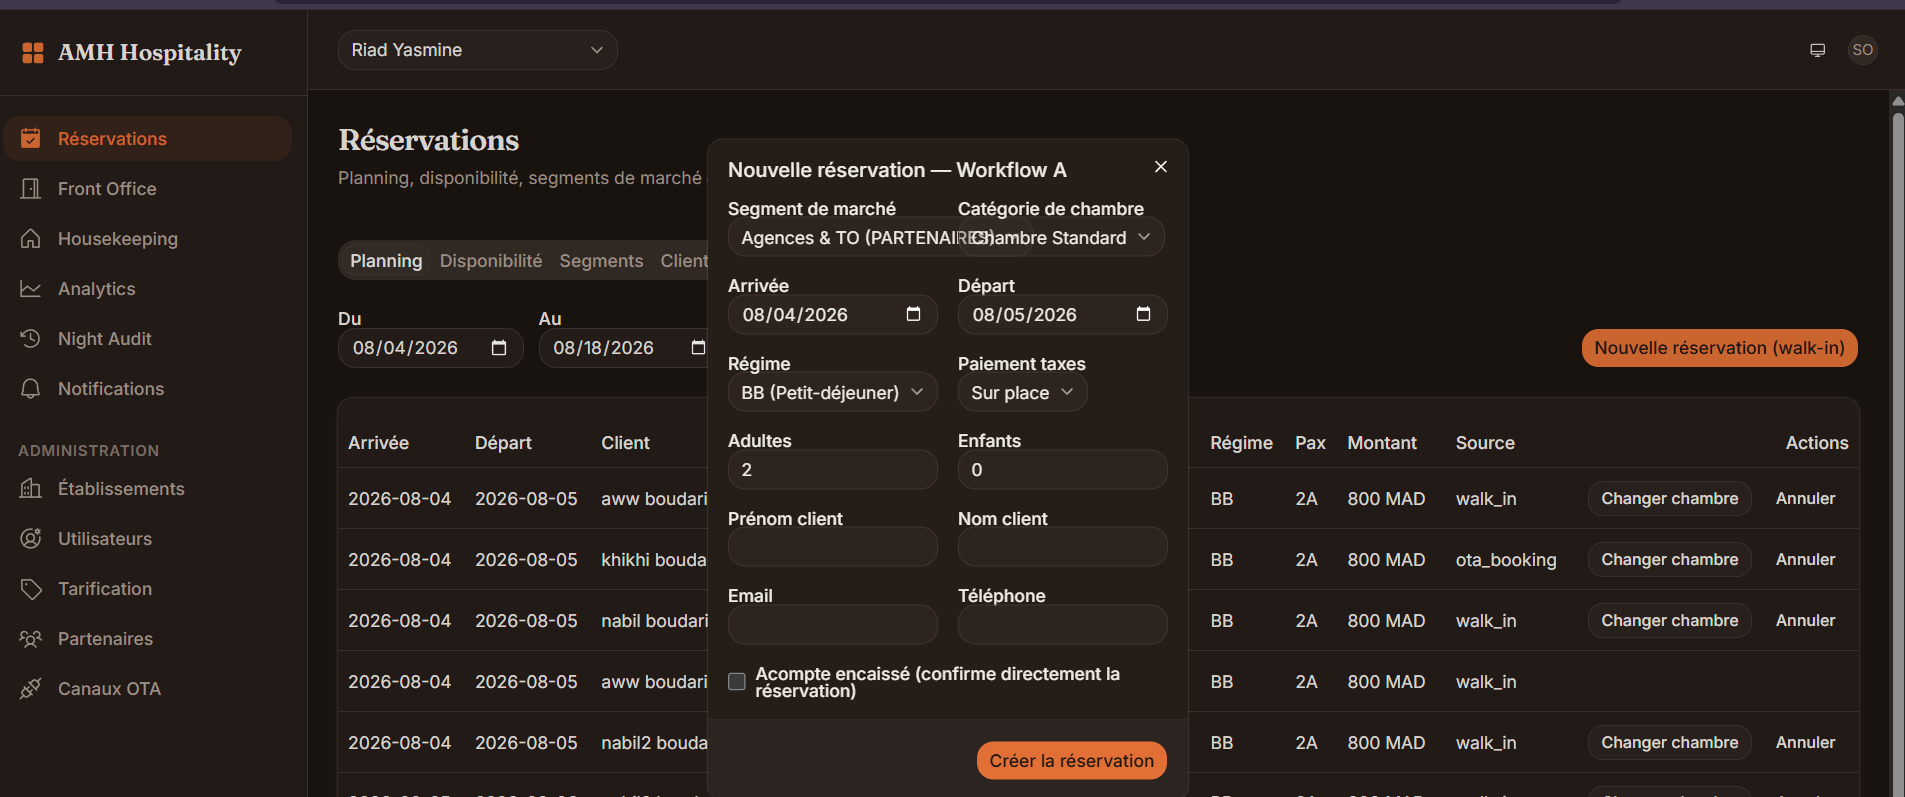
\includegraphics[width=0.9\textwidth]{figures/reservation.png}
\caption{Interface de création et modification de réservation}
\label{fig:reservation}
\end{figure}

Le formulaire (Figure~\ref{fig:reservation}) permet de renseigner les paramètres du séjour : sélection des dates d'arrivée et de départ via un calendrier interactif, choix de la catégorie de suite, nombre d'adultes et d'enfants, plan tarifaire et coordonnées du client. Dès l'ouverture du formulaire, le système acquiert un verrou distribué Redis sur la chambre ciblée pour garantir l'absence de conflit de concurrence.

\subsubsection{Interface de Check-in voyageur et formalités d'accueil}

La Figure~\ref{fig:checkin} et la Figure~\ref{fig:businescheckin} présentent les interfaces guidant le réceptionniste lors de l'arrivée du voyageur.

\begin{figure}[H]
\centering
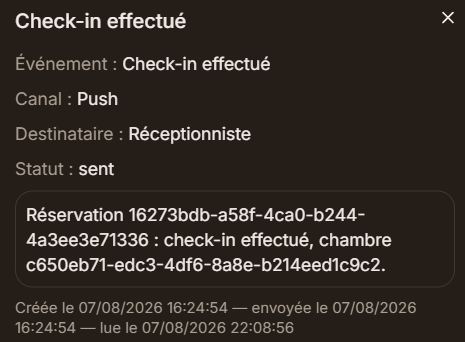
\includegraphics[width=0.85\textwidth]{figures/checkin.png}
\caption{Interface de Check-in voyageur et contrôle de propreté}
\label{fig:checkin}
\end{figure}

\begin{figure}[H]
\centering
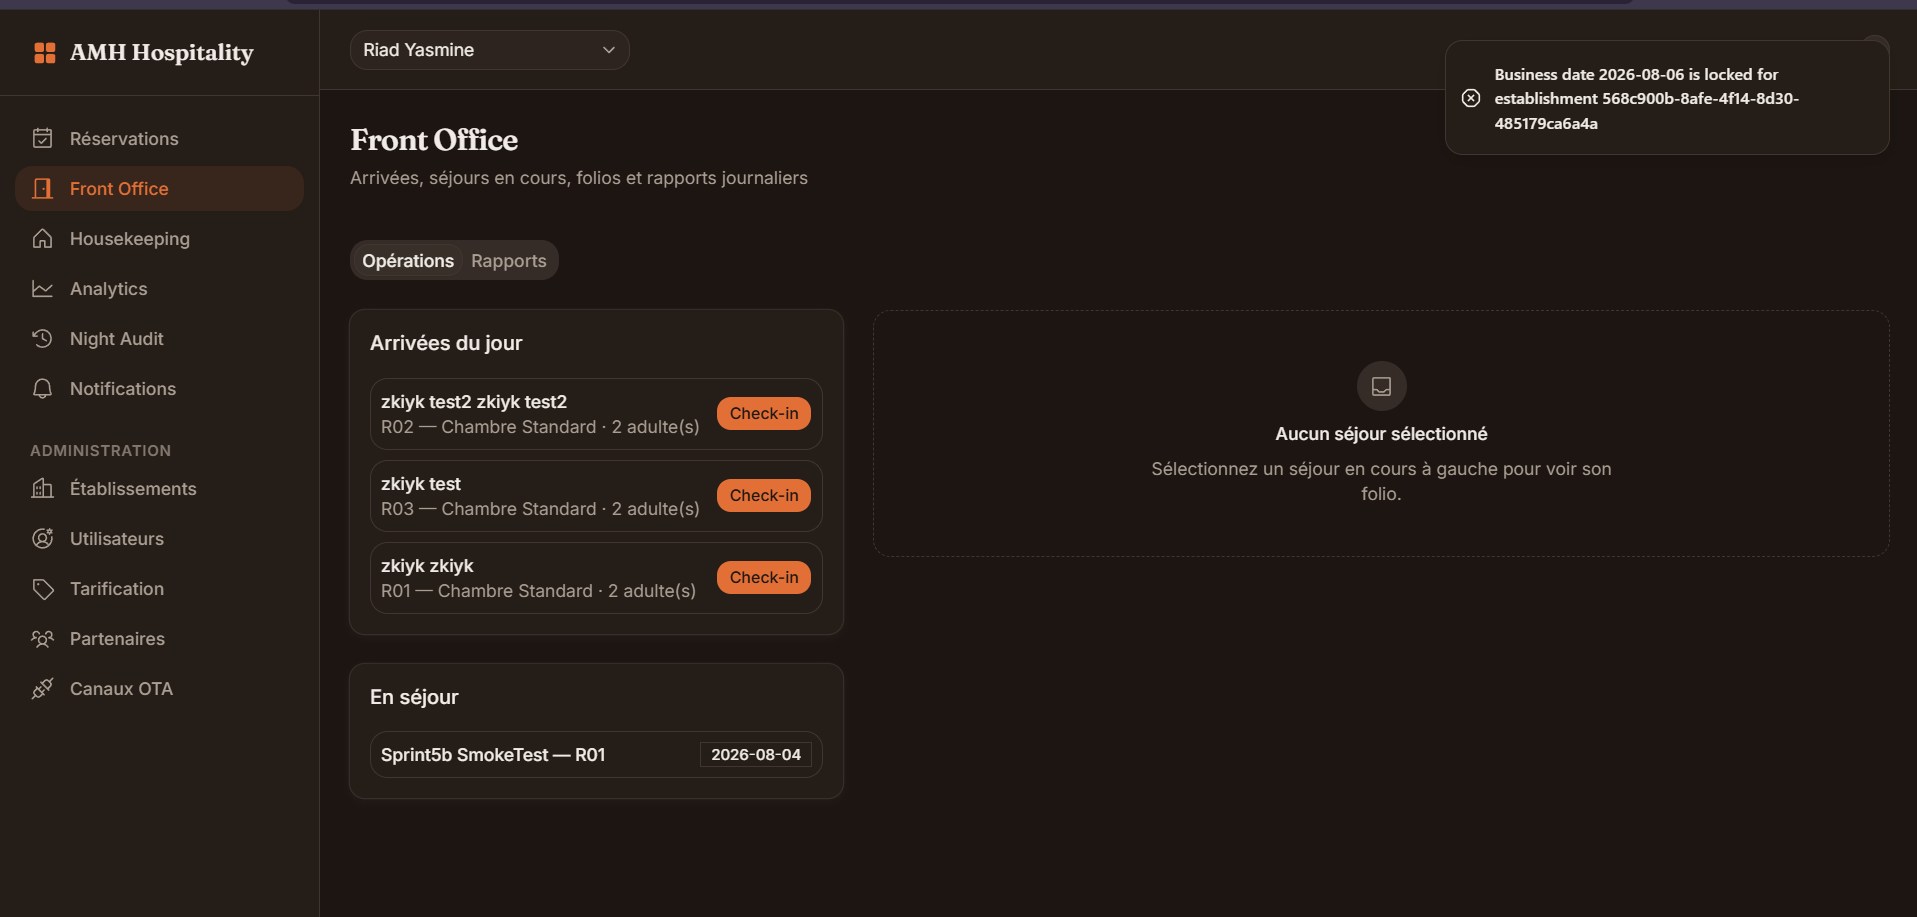
\includegraphics[width=0.9\textwidth]{figures/businescheckin.png}
\caption{Interface détaillée d'enregistrement des pièces d'identité (Fiche de police)}
\label{fig:businescheckin}
\end{figure}

Comme le montrent la Figure~\ref{fig:checkin} et la Figure~\ref{fig:businescheckin}, le processus de Check-in vérifie automatiquement que la suite assignée a bien été validée au statut \texttt{CLEAN} ou \texttt{INSPECTED} par la gouvernante. Le réceptionniste renseigne les pièces d'identité officielles du voyageur (numéro de passeport, date de délivrance et nationalité) nécessaires à la production de la fiche de police marocaine réglementaire, puis valide l'entrée qui bascule le séjour en \texttt{IN\_HOUSE}.

\subsubsection{Interface de visualisation des séjours actifs (In-House)}

La Figure~\ref{fig:zkiyk} présente la liste consolidée des clients séjournant actuellement dans le Riad.

\begin{figure}[H]
\centering
\includegraphics[width=0.85\textwidth]{figures/zkiyk.png}
\caption{Interface de consultation des séjours actifs (In-House)}
\label{fig:zkiyk}
\end{figure}

La Figure~\ref{fig:zkiyk} permet au chef de réception de suivre l'ensemble des dossiers actifs, d'accéder d'un clic aux folios correspondants et de visualiser les demandes particulières des résidents.

\subsection{Module 4 : Facturation, folios et clôture Night Audit}

\subsubsection{Interface de facturation et gestion des Folios clients}

La Figure~\ref{fig:folio_1} illustre l'état de compte financier détaillé d'un séjour.

\begin{figure}[H]
\centering
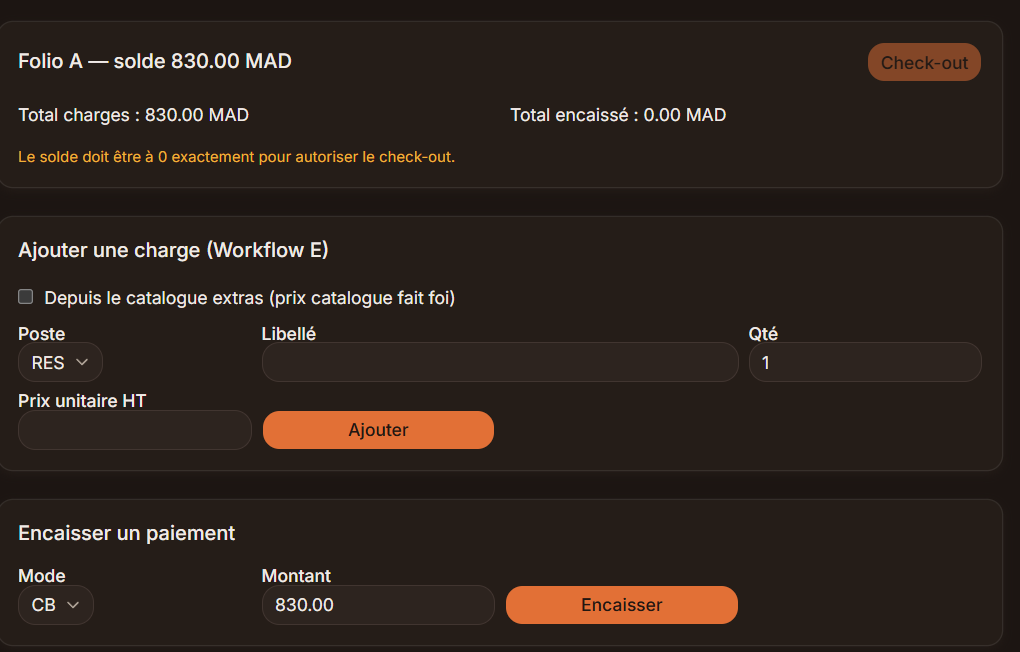
\includegraphics[width=0.9\textwidth]{figures/folio_1.png}
\caption{Interface de facturation et gestion des Folios clients}
\label{fig:folio_1}
\end{figure}

L'interface Folio (Figure~\ref{fig:folio_1}) centralise l'ensemble des mouvements financiers rattachés au séjour : débits correspondant aux nuitées d'hébergement, à la TVA (10\%), à la Taxe de Séjour communale (25 MAD/nuitée/personne), à la Taxe de Promotion Touristique (12 MAD/nuitée/personne) et aux extras imputés. Les crédits correspondent aux règlements enregistrés. La balance financière est calculée et affichée en temps réel avec solde net dû.

\subsubsection{Interface d'imputation des consommations et extras}

La Figure~\ref{fig:ajouter_charge} présente le modal d'ajout de prestations annexes sur le folio client.

\begin{figure}[H]
\centering
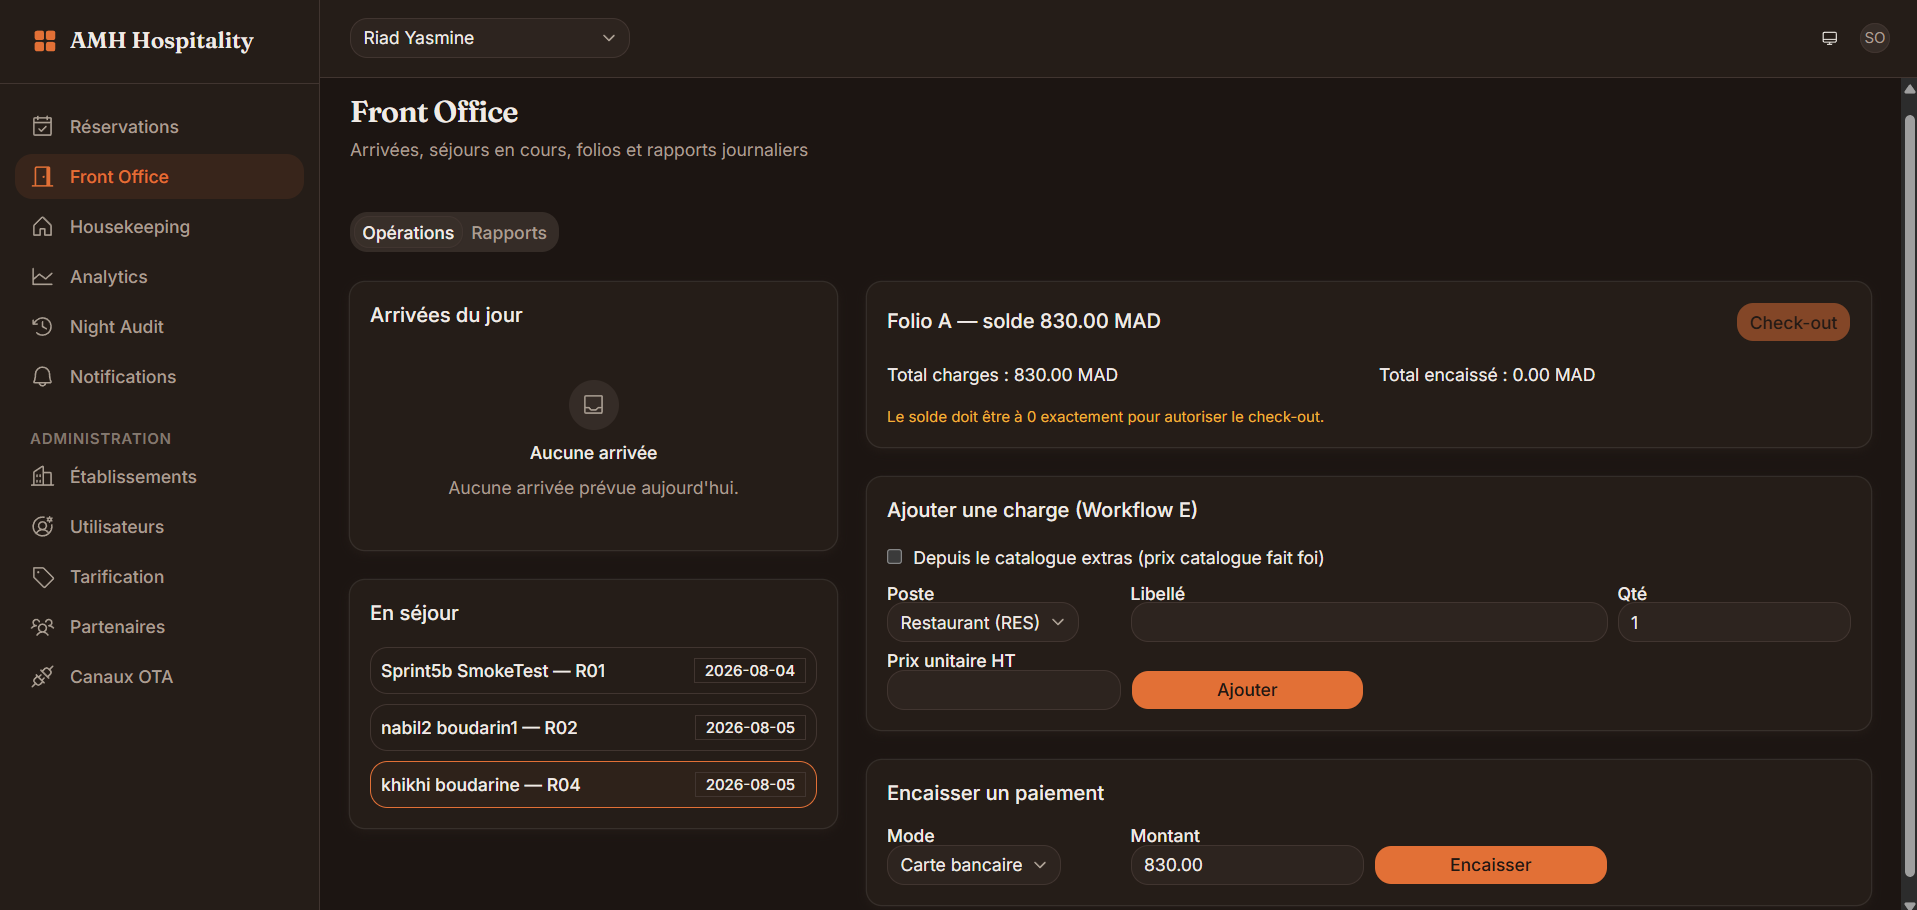
\includegraphics[width=0.85\textwidth]{figures/ajouter_charge.png}
\caption{Interface d'imputation des extras et consommations (Restaurant / Spa)}
\label{fig:ajouter_charge}
\end{figure}

La Figure~\ref{fig:ajouter_charge} permet au personnel de réception ou de restauration d'imputer des consommations directes : repas à la table d'hôtes, rituels de hammam/spa, transferts aéroport ou excursions, avec ventilation automatique du taux de TVA approprié et mise à jour instantanée du solde du folio.

\subsubsection{Interface de gestion de la Business Date et moteur de Night Audit}

La Figure~\ref{fig:business_date} présente le module de clôture journalière automatisée.

\begin{figure}[H]
\centering
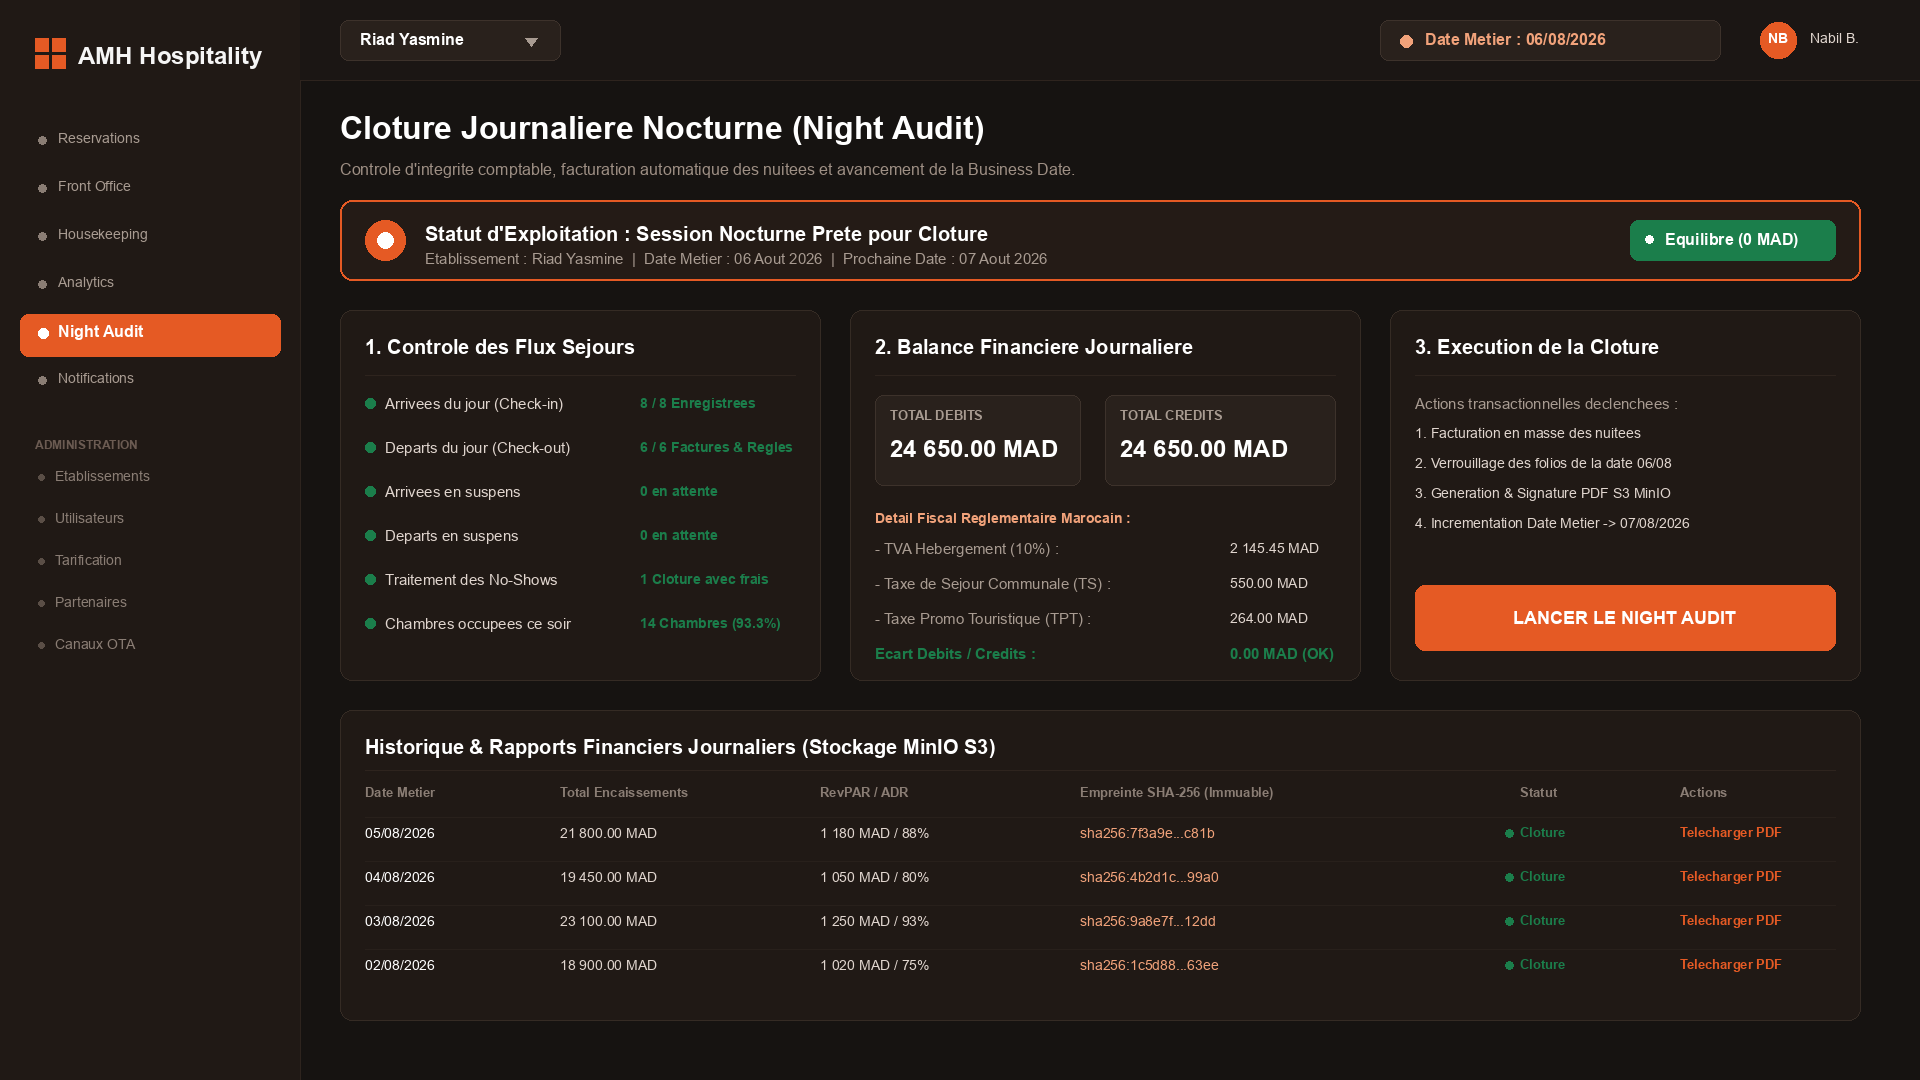
\includegraphics[width=0.9\textwidth]{figures/business_date.png}
\caption{Interface de gestion de la Business Date et clôture Night Audit}
\label{fig:business_date}
\end{figure}

La Figure~\ref{fig:business_date} est l'écran dédié à l'auditeur de nuit. Il présente la date d'exploitation active (\textit{Business Date}), le récapitulatif des contrôles de cohérence préalables et le bouton de déclenchement de la clôture automatisée. En un clic, le système exécute la facturation en masse de toutes les nuitées, génère le rapport PDF certifié, l'archive sur MinIO S3 et incrémente la date d'exploitation en seulement 45 secondes.

\subsection{Module 5 : Application mobile PWA Housekeeping et gouvernance d'étage}

La Figure~\ref{fig:femme} et la Figure~\ref{fig:mob} illustrent l'application mobile progressive dédiée aux équipes d'étage.

\begin{figure}[H]
\centering
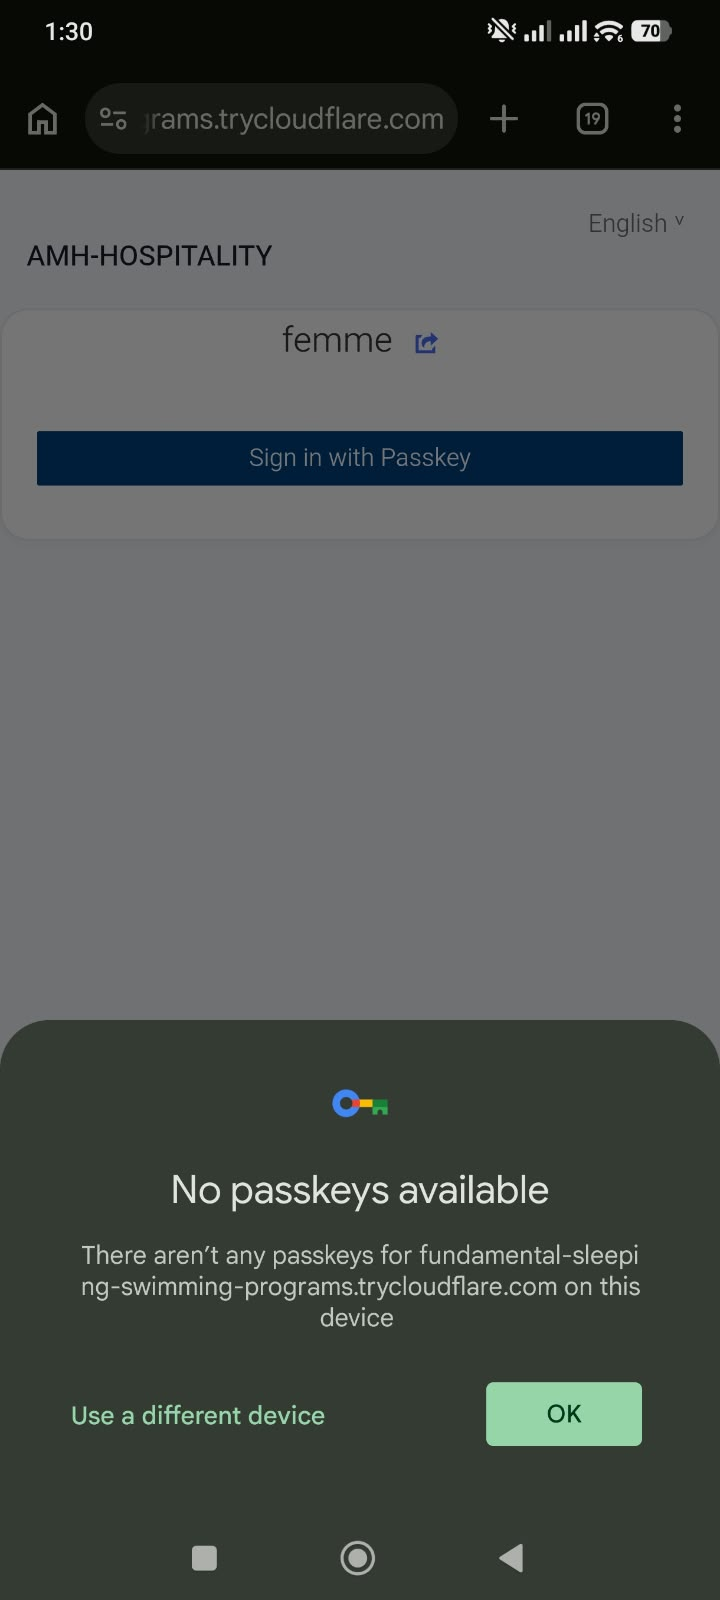
\includegraphics[width=0.5\textwidth]{figures/femme.jpeg}
\caption{Interface mobile PWA Housekeeping pour gouvernantes et femmes de chambre}
\label{fig:femme}
\end{figure}

\begin{figure}[H]
\centering
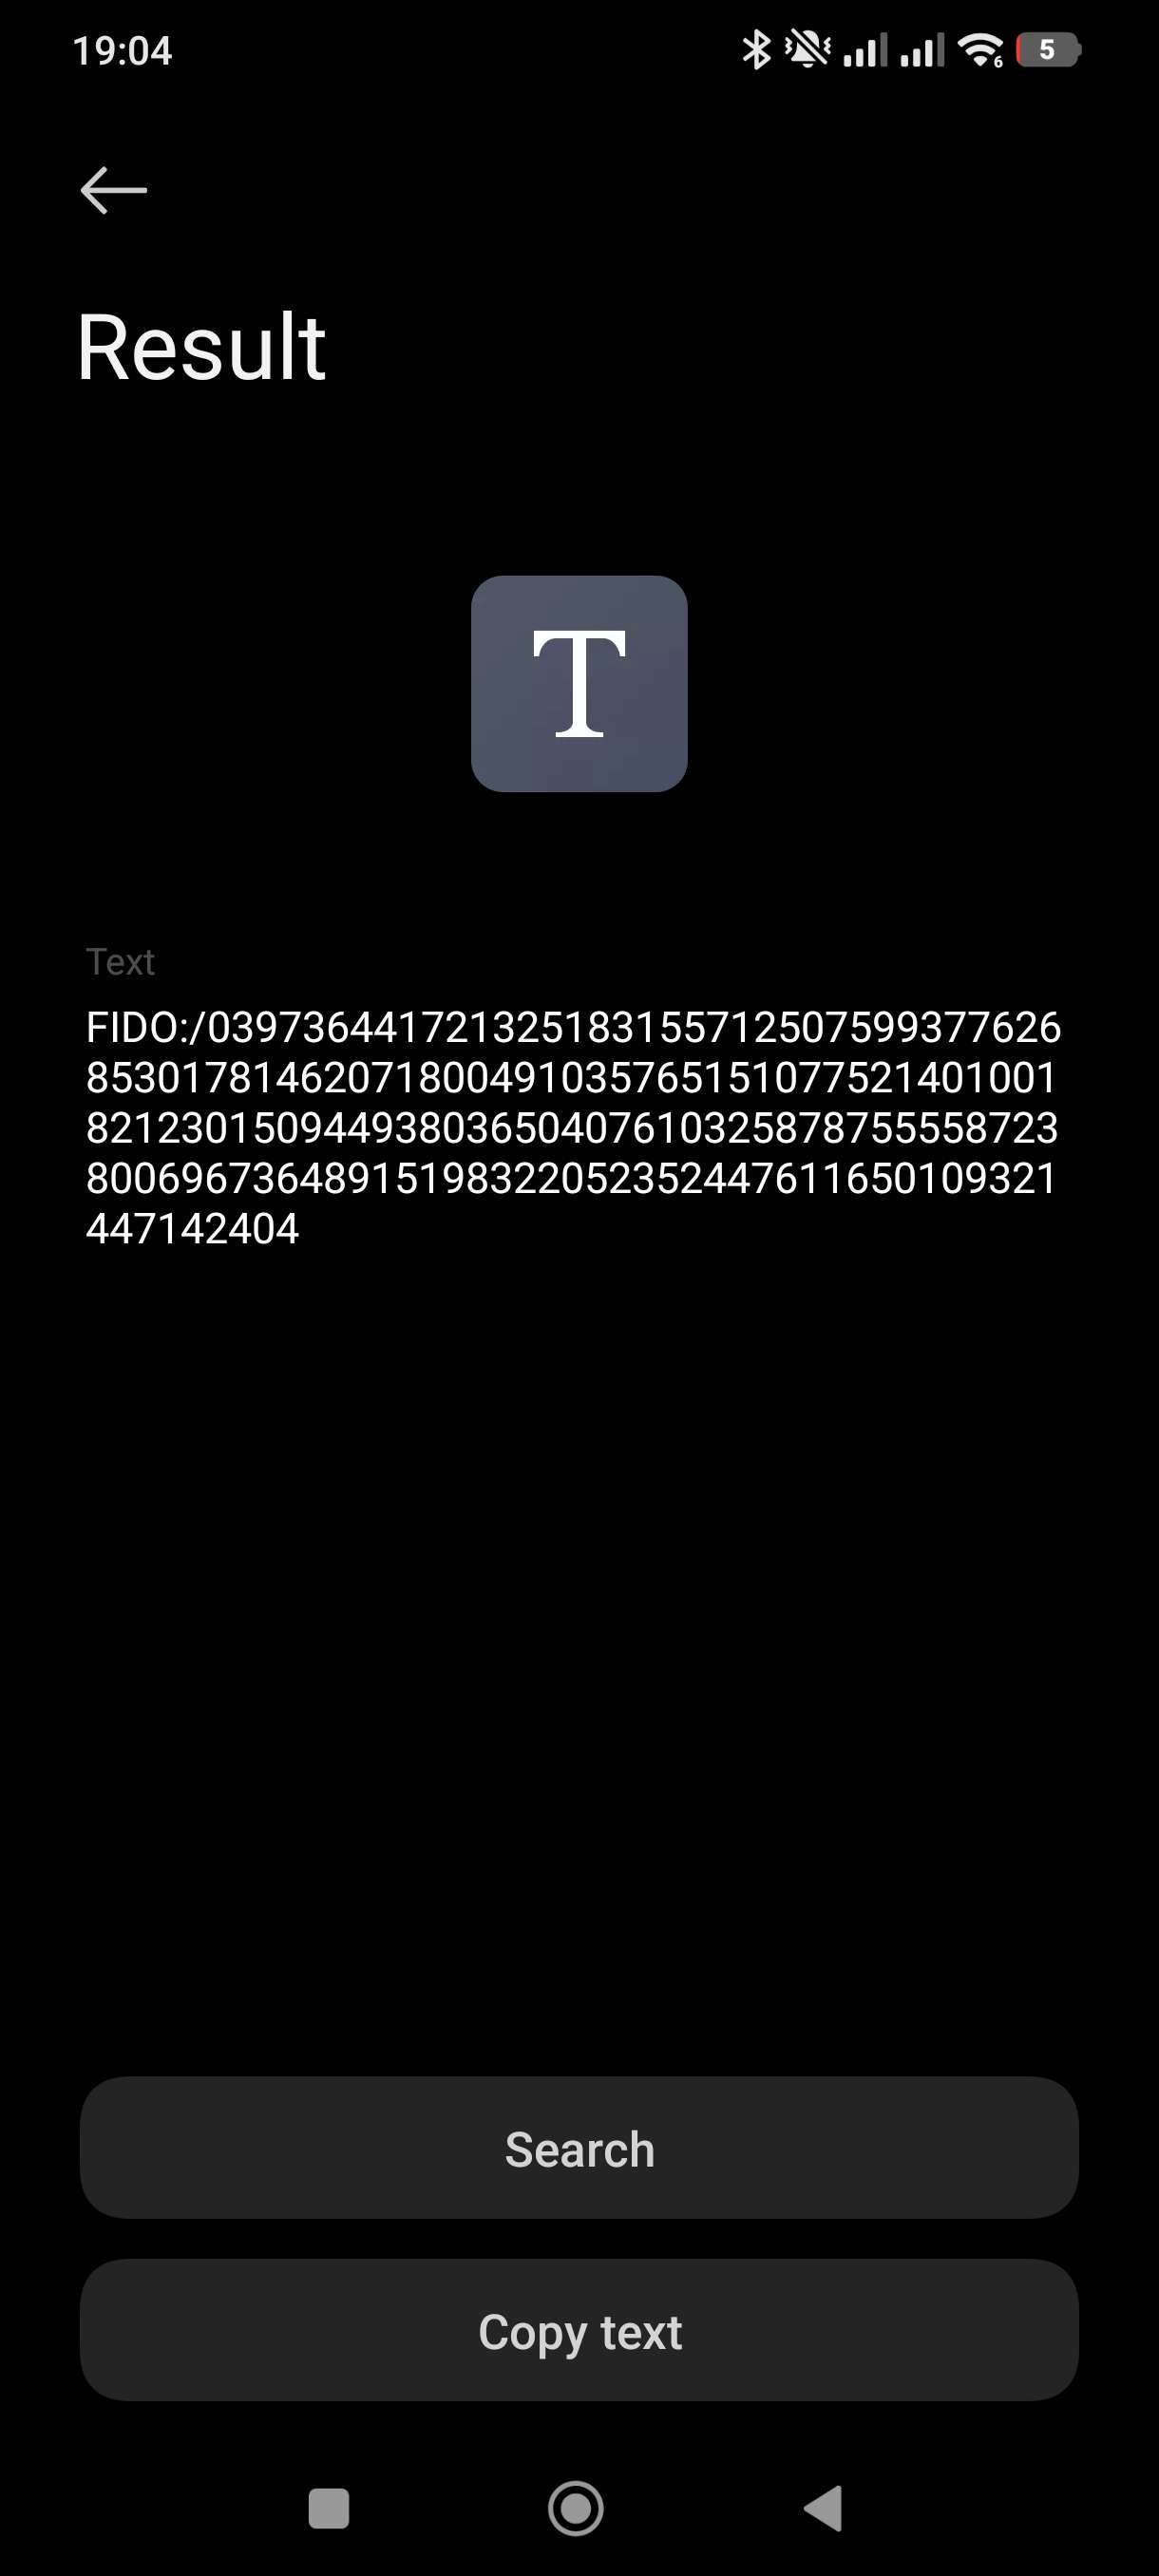
\includegraphics[width=0.5\textwidth]{figures/mob.jpg}
\caption{Vue mobile responsive de la plateforme PMS}
\label{fig:mob}
\end{figure}

Comme le montrent la Figure~\ref{fig:femme} et la Figure~\ref{fig:mob}, la PWA Housekeeping s'exécute sur n'importe quel smartphone sans installation depuis un store d'applications. Les femmes de chambre y consultent la liste ordonnée de leurs chambres assignées. Un appui sur un bouton permet de faire passer une chambre de l'état \texttt{DIRTY} à \texttt{CLEANING\_IN\_PROGRESS}, puis à \texttt{CLEAN}. Dès validation par la gouvernante au statut \texttt{INSPECTED}, l'information est répercutée en moins de 3 secondes sur le Tape Chart de réception via WebSockets.

\subsection{Module 6 : Administration multi-établissements, clients et notifications}

\subsubsection{Interface de gestion multi-établissements (Riads du groupe)}

La Figure~\ref{fig:etabli} présente l'interface d'administration multi-propriétés.

\begin{figure}[H]
\centering
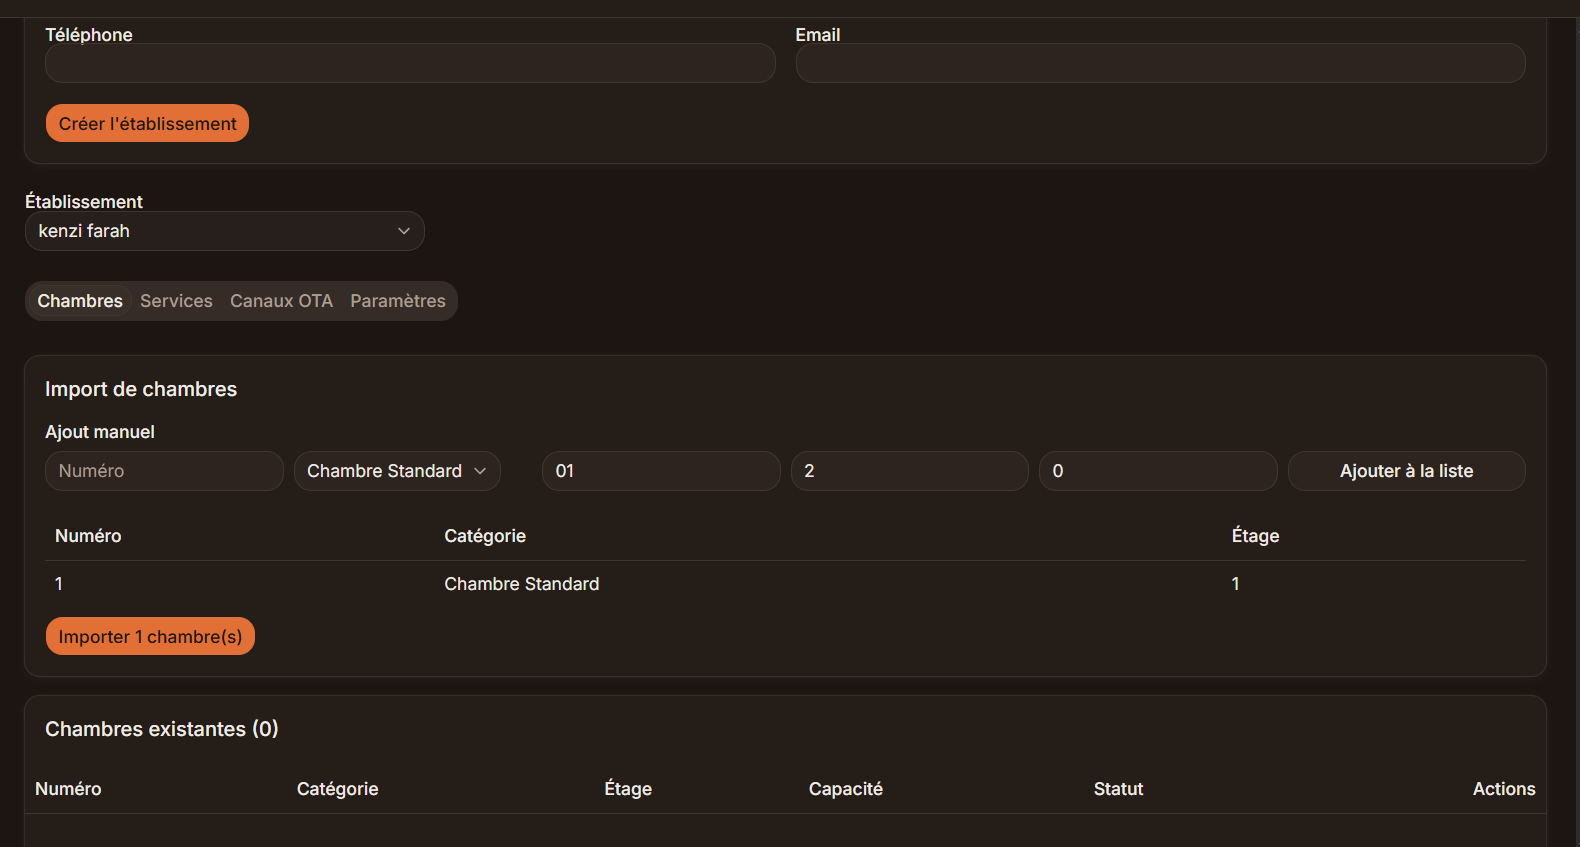
\includegraphics[width=0.85\textwidth]{figures/etabli.png}
\caption{Interface de gestion multi-établissements (Riads et Hôtels)}
\label{fig:etabli}
\end{figure}

La Figure~\ref{fig:etabli} permet à la direction générale de superviser l'ensemble des établissements du groupe AMH, d'en créer de nouveaux, de paramétrer les catégories de chambres et de configurer les taux fiscaux spécifiques à chaque commune.

\subsubsection{Interface Répertoire et fiches de profils clients}

La Figure~\ref{fig:names} et la Figure~\ref{fig:clients} présentent l'annuaire unifié des voyageurs.

\begin{figure}[H]
\centering
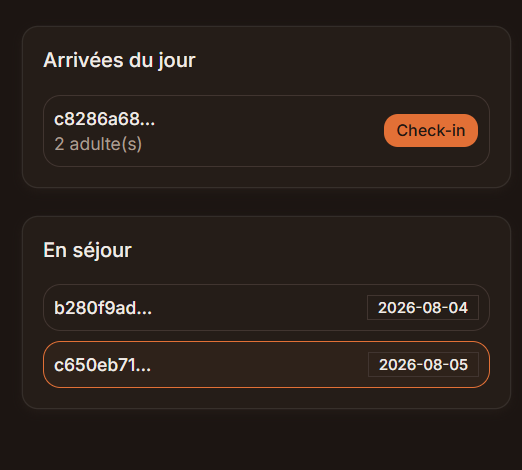
\includegraphics[width=0.85\textwidth]{figures/names.png}
\caption{Interface Répertoire et fiches profils clients}
\label{fig:names}
\end{figure}

\begin{figure}[H]
\centering
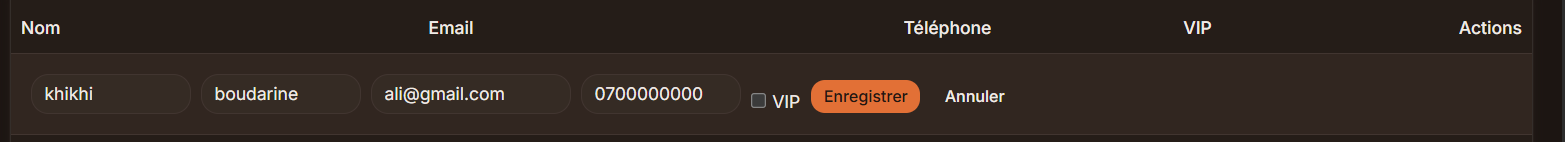
\includegraphics[width=0.85\textwidth]{figures/clients.png}
\caption{Vue détaillée de la base de données voyageurs et segmentation VIP}
\label{fig:clients}
\end{figure}

La Figure~\ref{fig:names} et la Figure~\ref{fig:clients} permettent de centraliser les historiques de séjours de chaque client à travers l'ensemble des Riads du groupe, d'enregistrer leurs préférences (chambre calme, régime alimentaire) et d'adapter l'accueil selon leur statut VIP.

\subsubsection{Interface Centre de notifications et alertes temps réel}

La Figure~\ref{fig:notifs_bell} et la Figure~\ref{fig:notifs_state} illustrent le centre de notifications événementielles.

\begin{figure}[H]
\centering
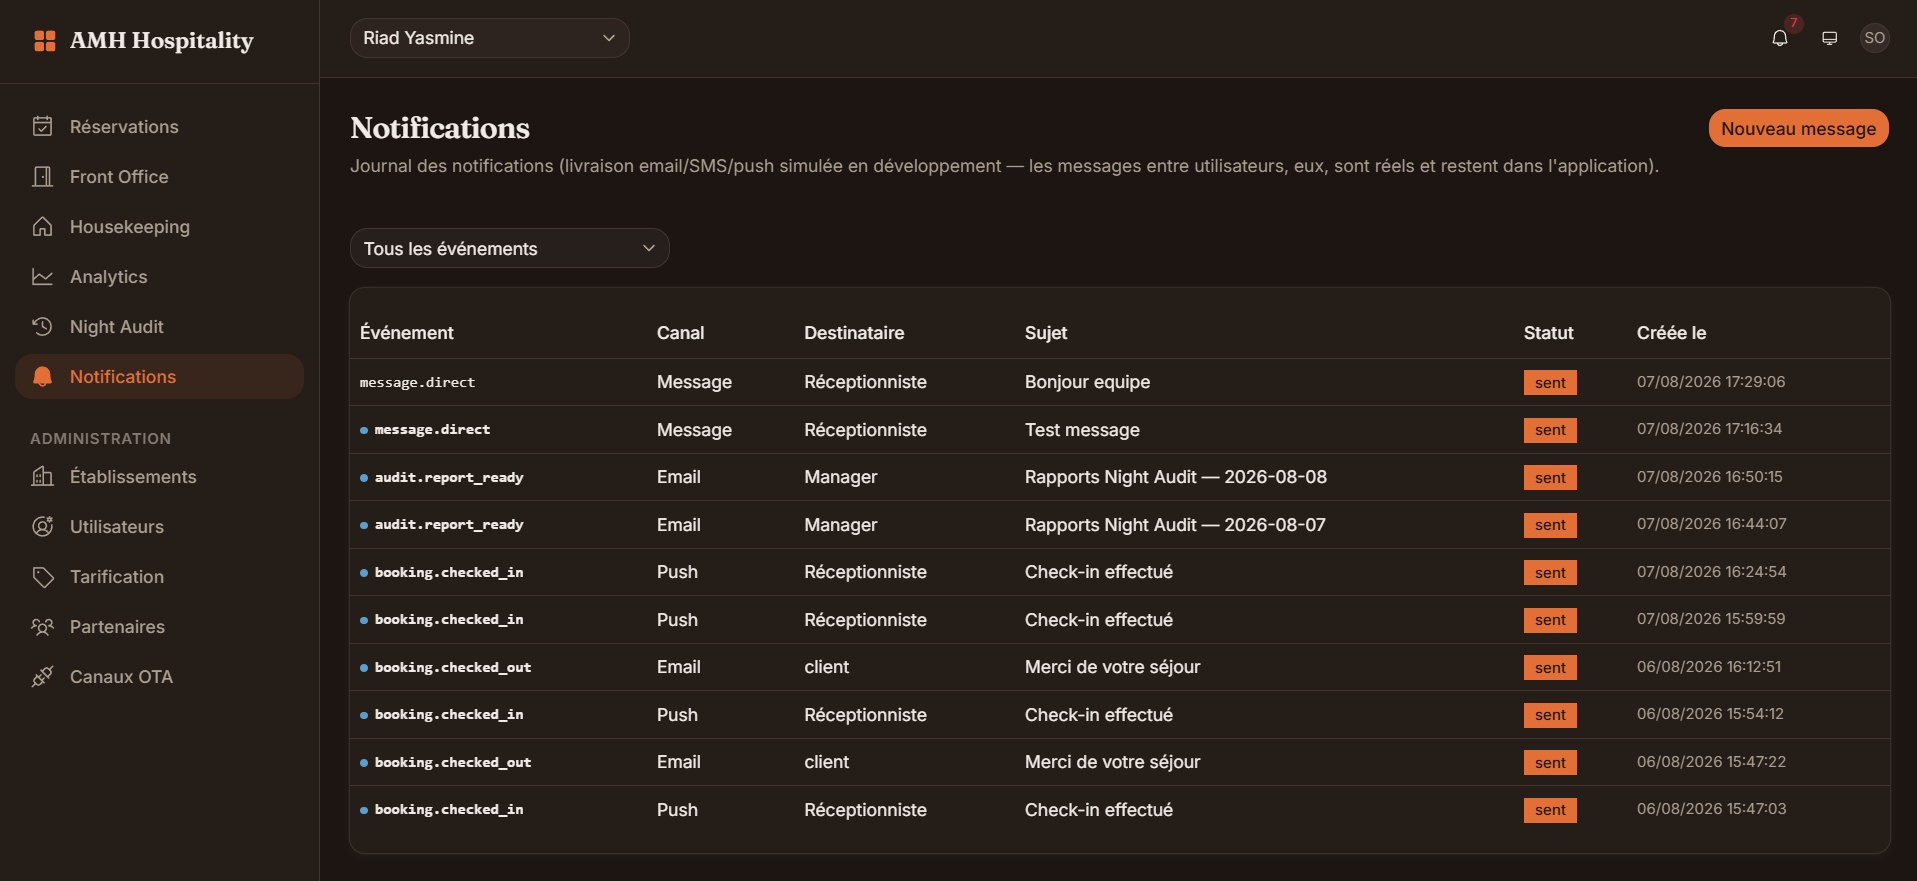
\includegraphics[width=0.75\textwidth]{figures/notifications-page-topbar-bell.png}
\caption{Interface Centre de notifications et alertes temps réel}
\label{fig:notifs_bell}
\end{figure}

\begin{figure}[H]
\centering
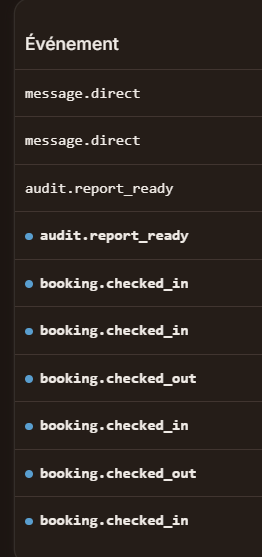
\includegraphics[width=0.85\textwidth]{figures/notifications-event-column-read-unread-state.png}
\caption{Gestion des états de lecture et priorités des notifications}
\label{fig:notifs_state}
\end{figure}

La Figure~\ref{fig:notifs_bell} et la Figure~\ref{fig:notifs_state} affichent les alertes diffusées par le bus RabbitMQ : arrivées imminentes, chambres prêtes, alertes de solde débiteur et clôtures nocturnes réussies.

\subsubsection{Interfaces de gestion des erreurs transactionnelles et guidage}

La Figure~\ref{fig:err_toast}, la Figure~\ref{fig:req_failed}, la Figure~\ref{fig:req_failed_2} et la Figure~\ref{fig:echec} présentent les mécanismes de retour visuel lors des anomalies opérationnelles.

\begin{figure}[H]
\centering
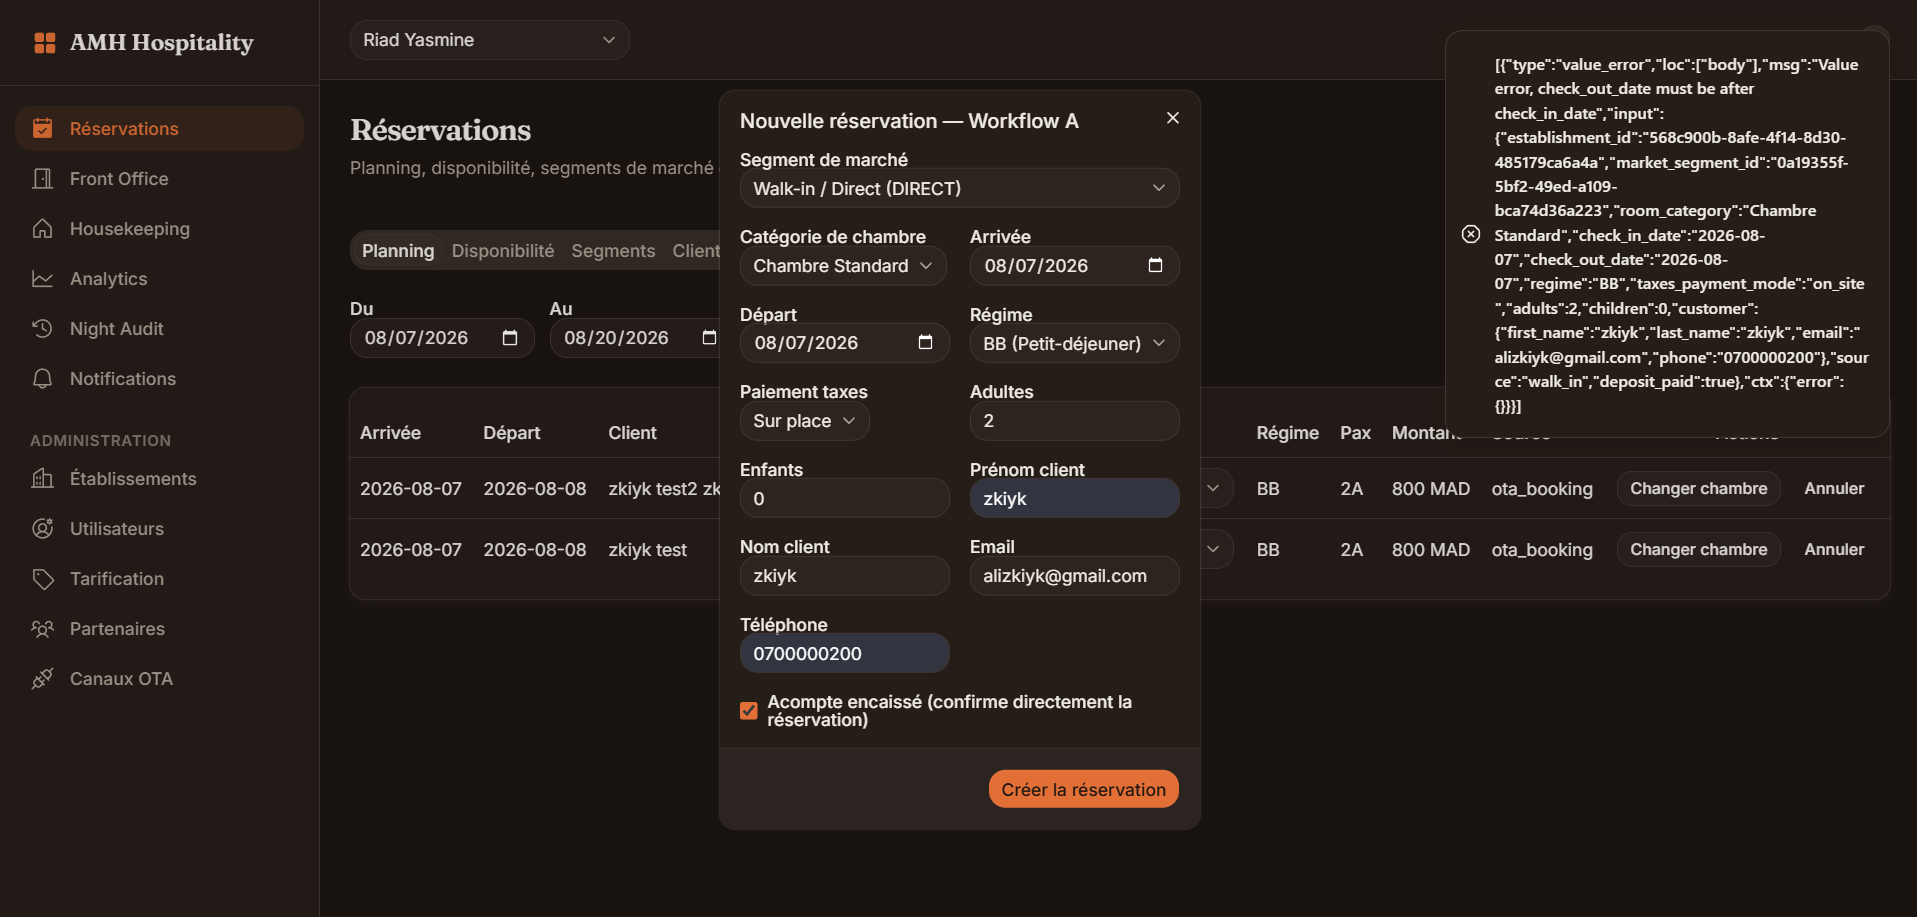
\includegraphics[width=0.85\textwidth]{figures/reservation-create-error-toast.png}
\caption{Notification visuelle (Toast) de rejet de réservation concurrente}
\label{fig:err_toast}
\end{figure}

\begin{figure}[H]
\centering
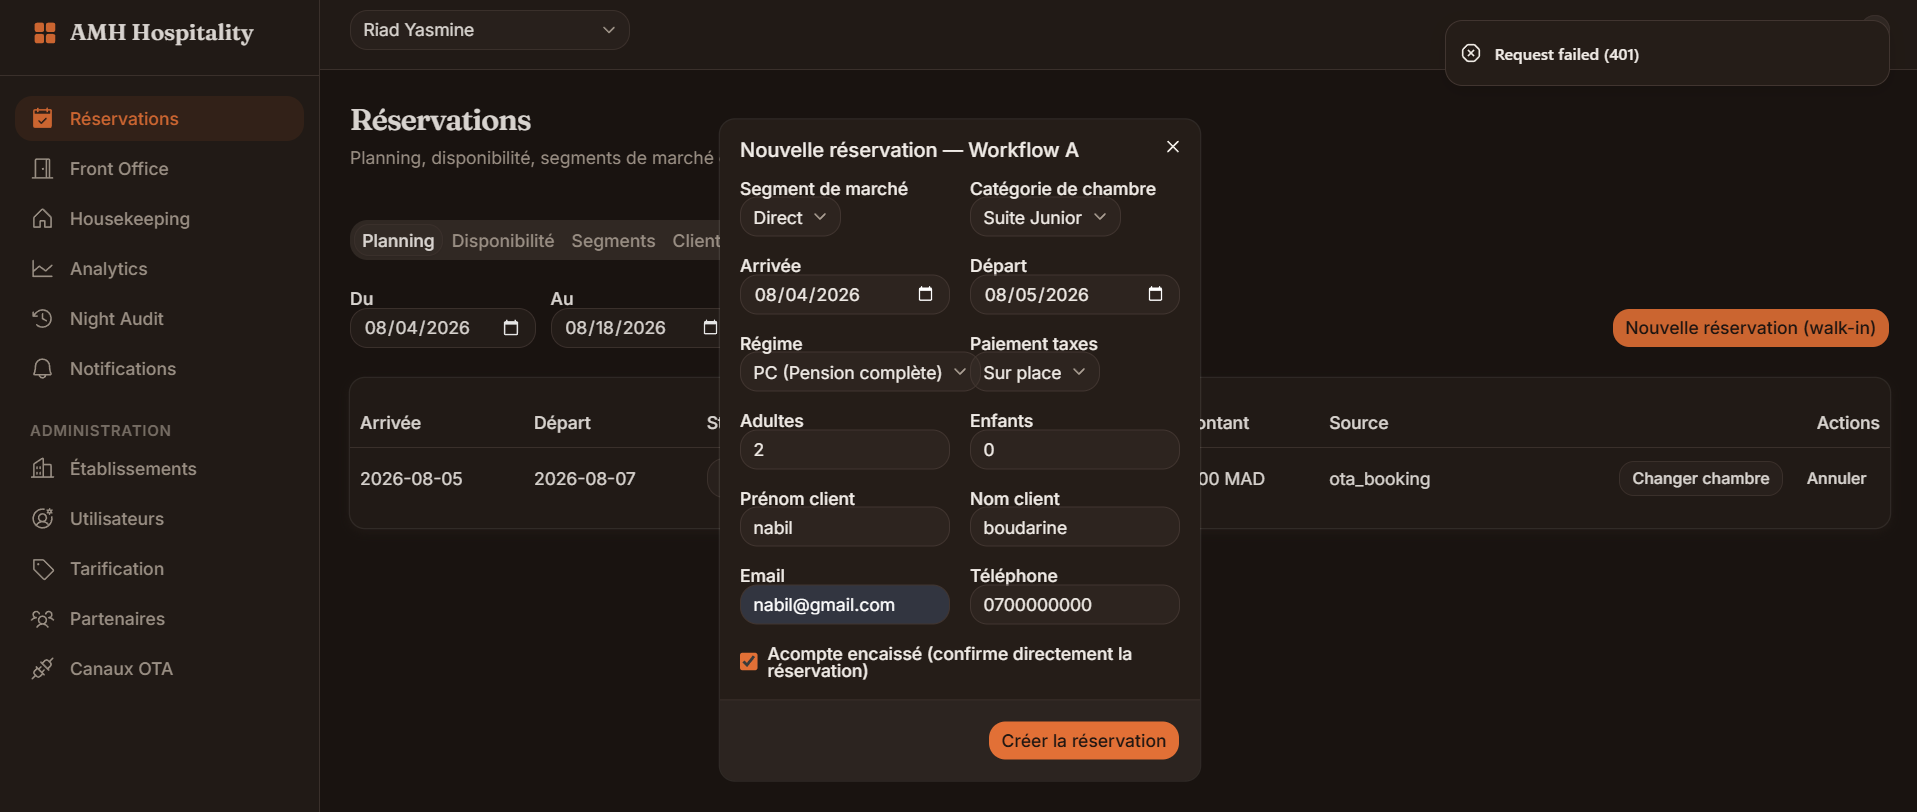
\includegraphics[width=0.85\textwidth]{figures/request_failed.png}
\caption{Interface de gestion des erreurs de communication réseau}
\label{fig:req_failed}
\end{figure}

\begin{figure}[H]
\centering
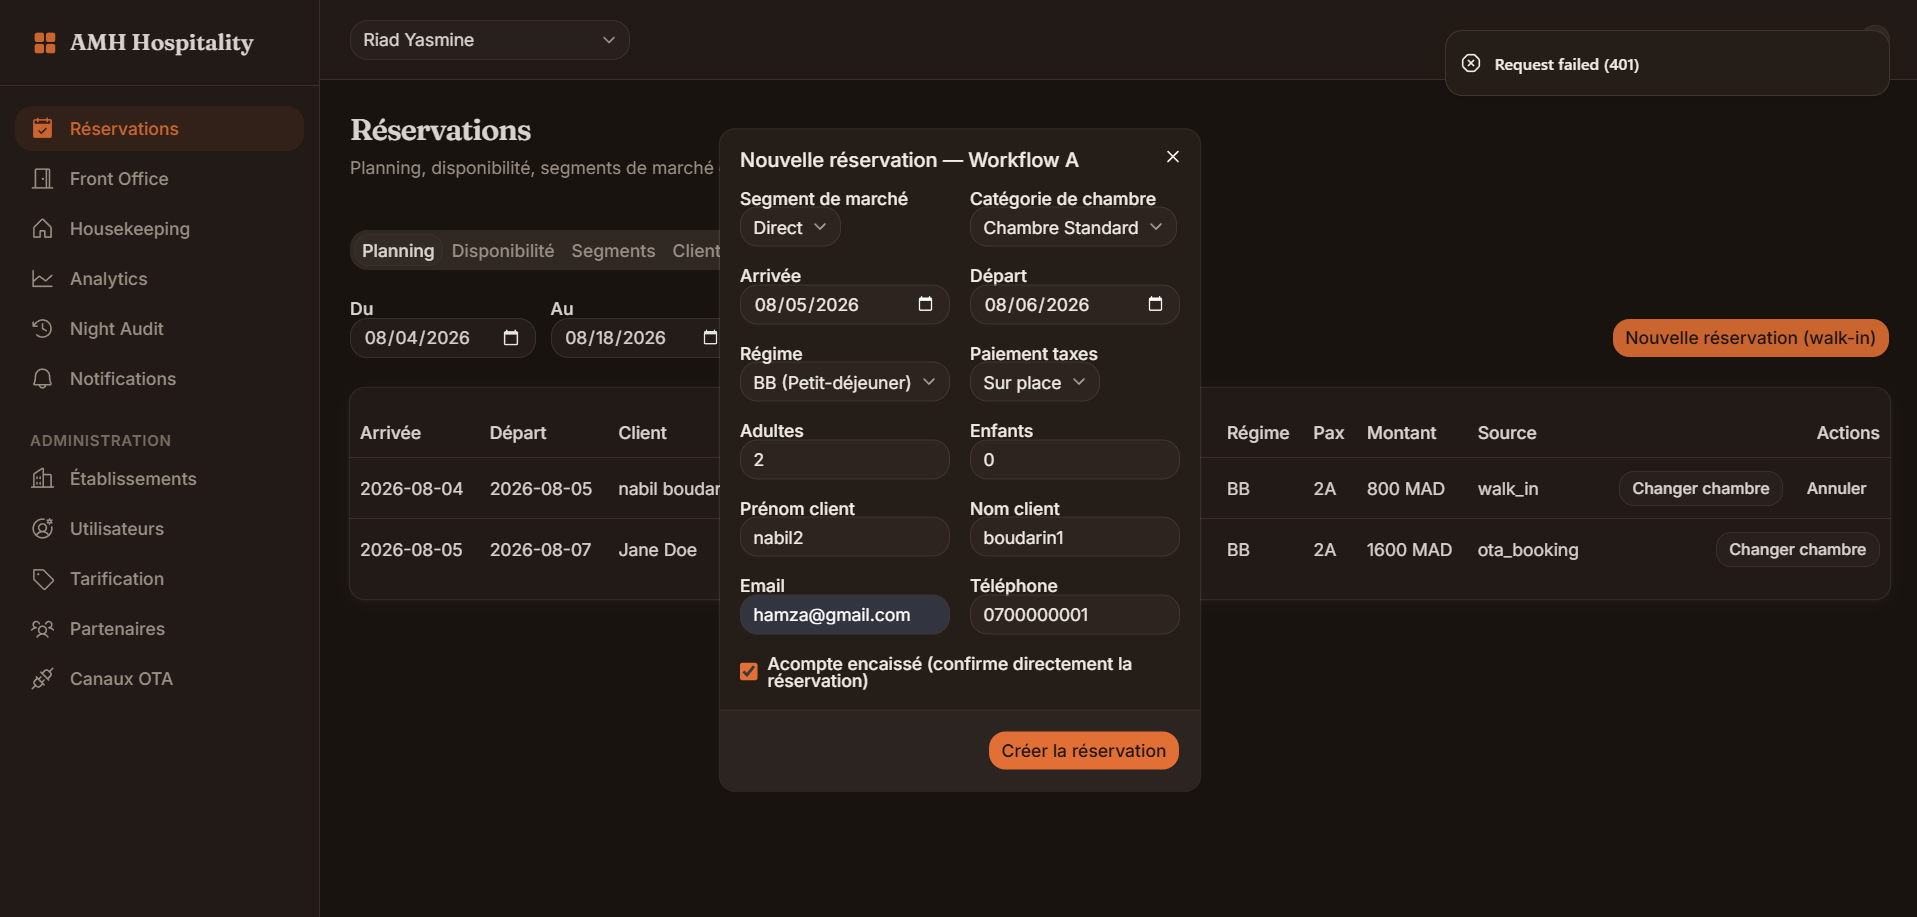
\includegraphics[width=0.85\textwidth]{figures/request_failed_2.png}
\caption{Interface explicative des erreurs de validation des schémas Pydantic}
\label{fig:req_failed_2}
\end{figure}

\begin{figure}[H]
\centering
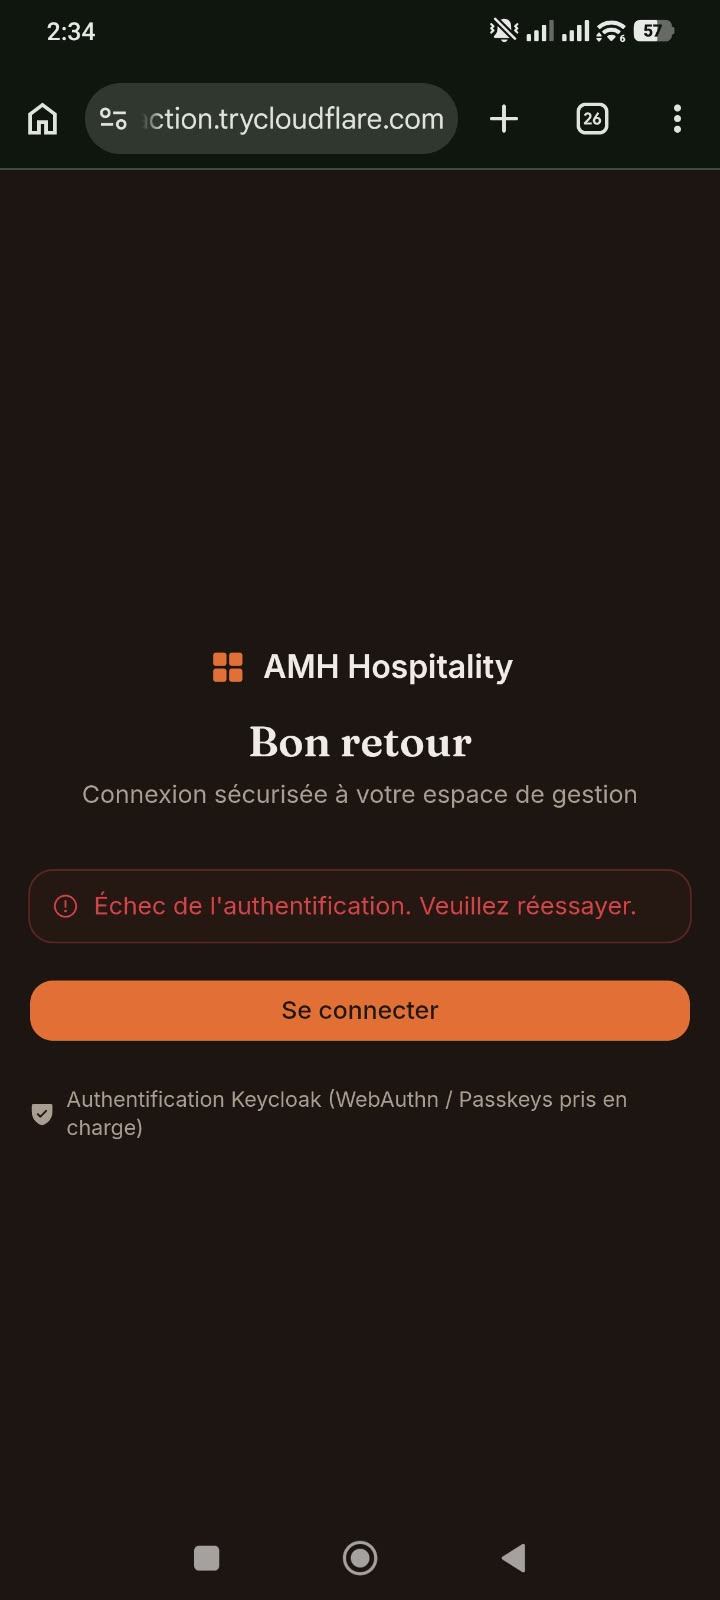
\includegraphics[width=0.85\textwidth]{figures/echec.jpeg}
\caption{Écran d'échec de transaction financière et propositions de résolution}
\label{fig:echec}
\end{figure}

Ces interfaces assurent un guidage sans ambiguïté pour le personnel en cas de fausse manipulation ou de conflit réseau.

\subsubsection{Interfaces de communication, requêtes et supervision}

La Figure~\ref{fig:news}, la Figure~\ref{fig:rq}, la Figure~\ref{fig:logs} et la Figure~\ref{fig:pic7} présentent les modules complémentaires d'exploitation.

\begin{figure}[H]
\centering
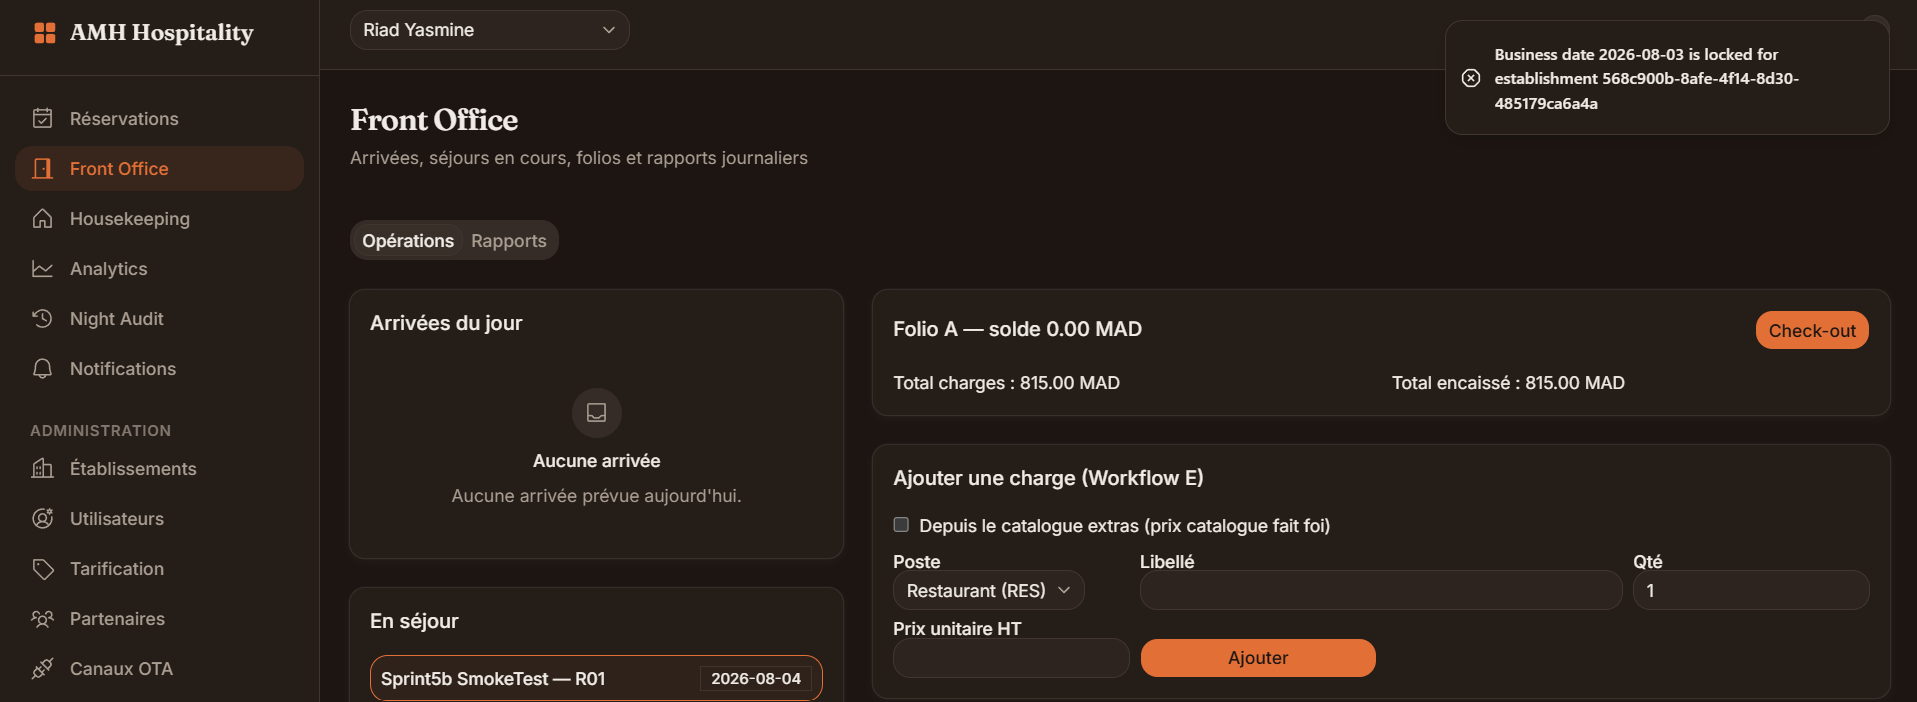
\includegraphics[width=0.85\textwidth]{figures/news.png}
\caption{Interface de gestion des actualités et consignes internes du Riad}
\label{fig:news}
\end{figure}

\begin{figure}[H]
\centering
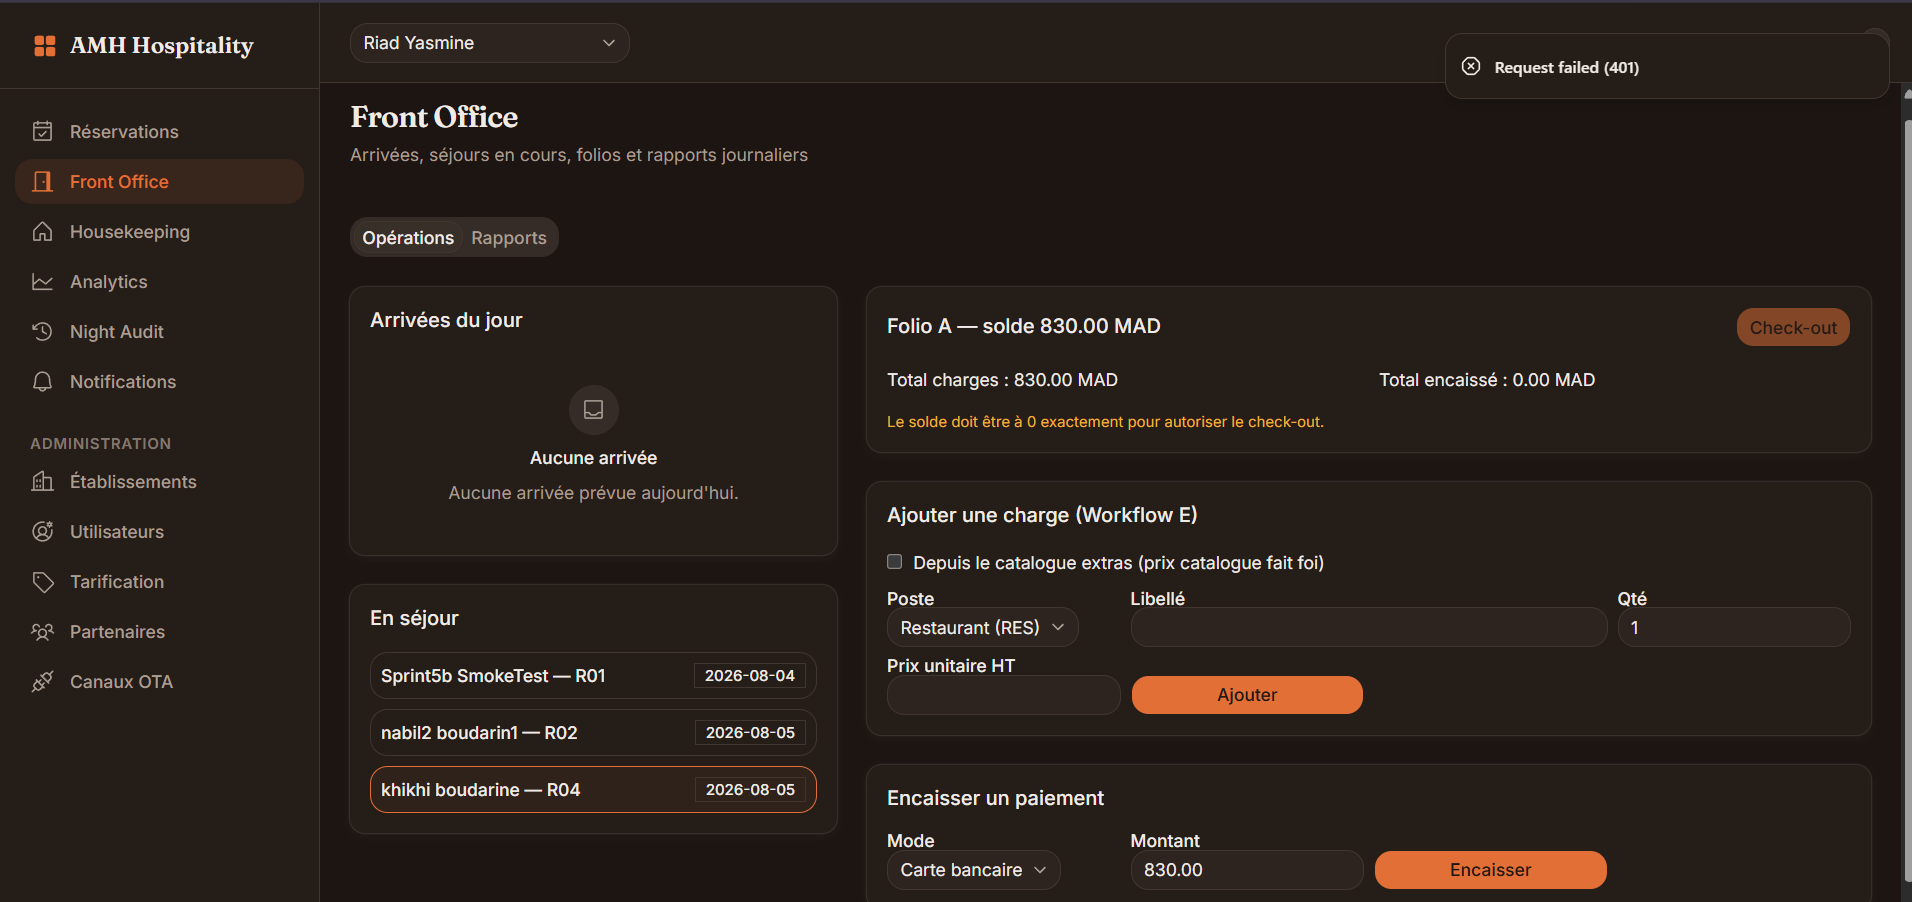
\includegraphics[width=0.85\textwidth]{figures/rq.png}
\caption{Interface de traitement des requêtes et demandes d'assistance}
\label{fig:rq}
\end{figure}

\begin{figure}[H]
\centering
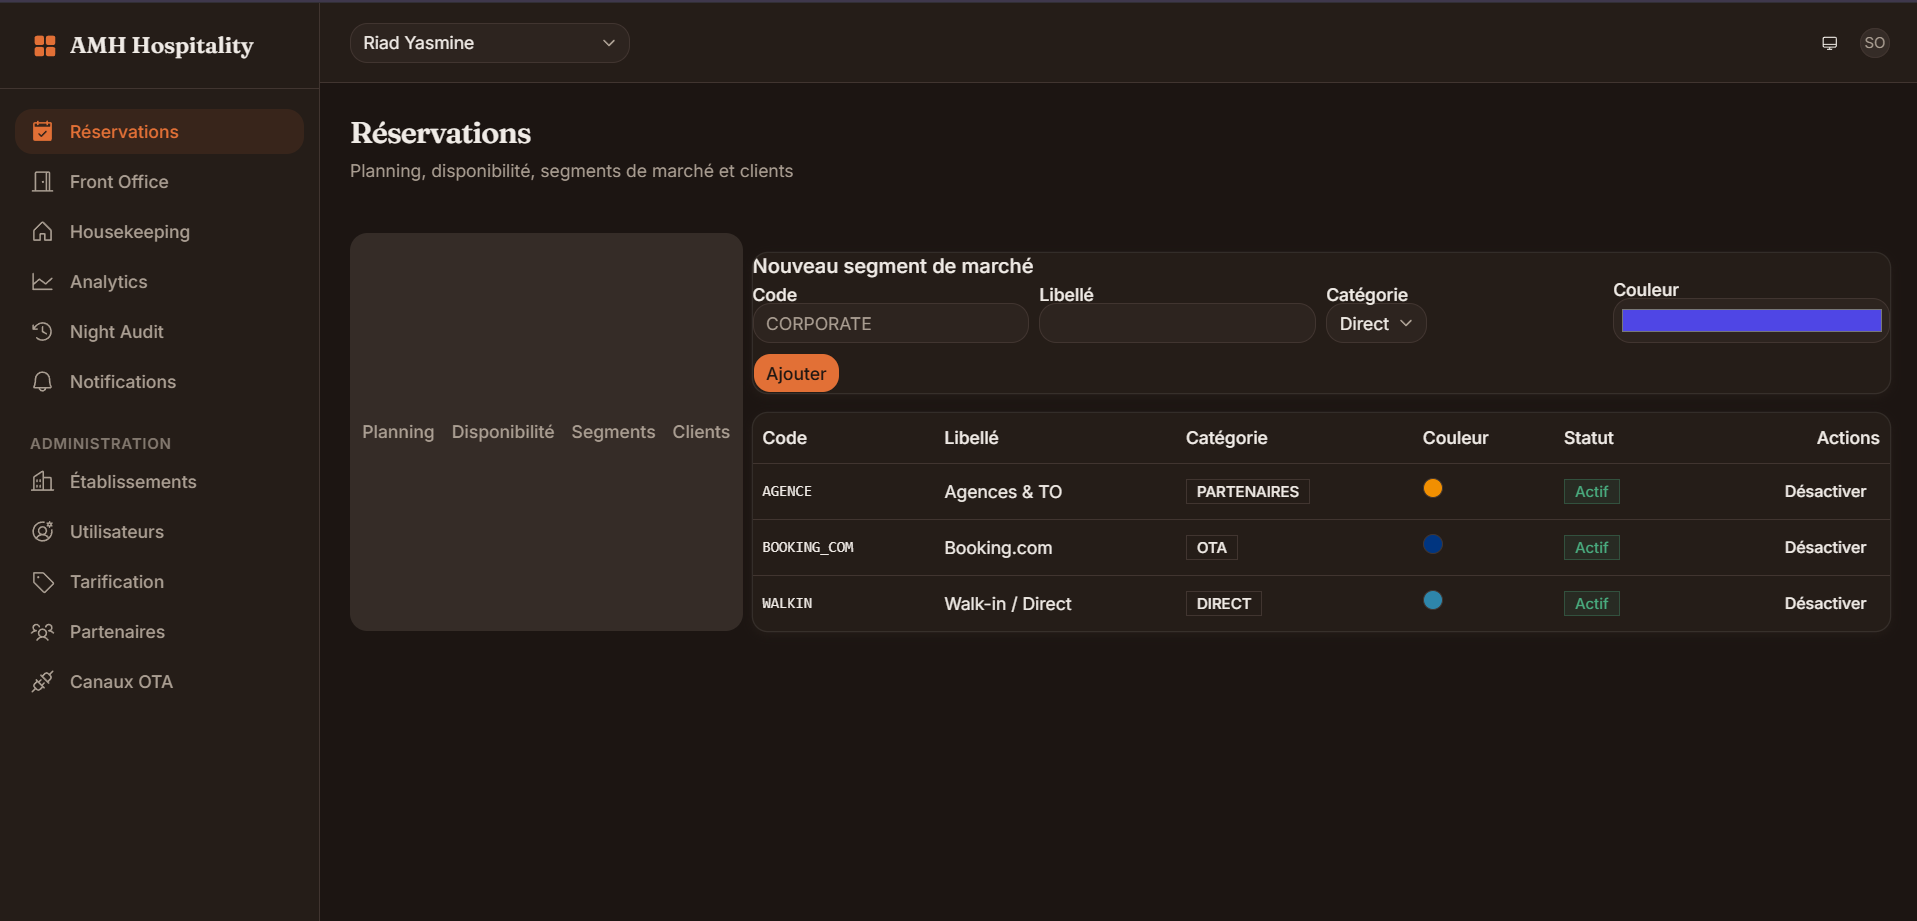
\includegraphics[width=0.85\textwidth]{figures/screenshot_2026-08-03_224130.png}
\caption{Interface de monitoring des logs d'exécution des microservices}
\label{fig:logs}
\end{figure}

\begin{figure}[H]
\centering
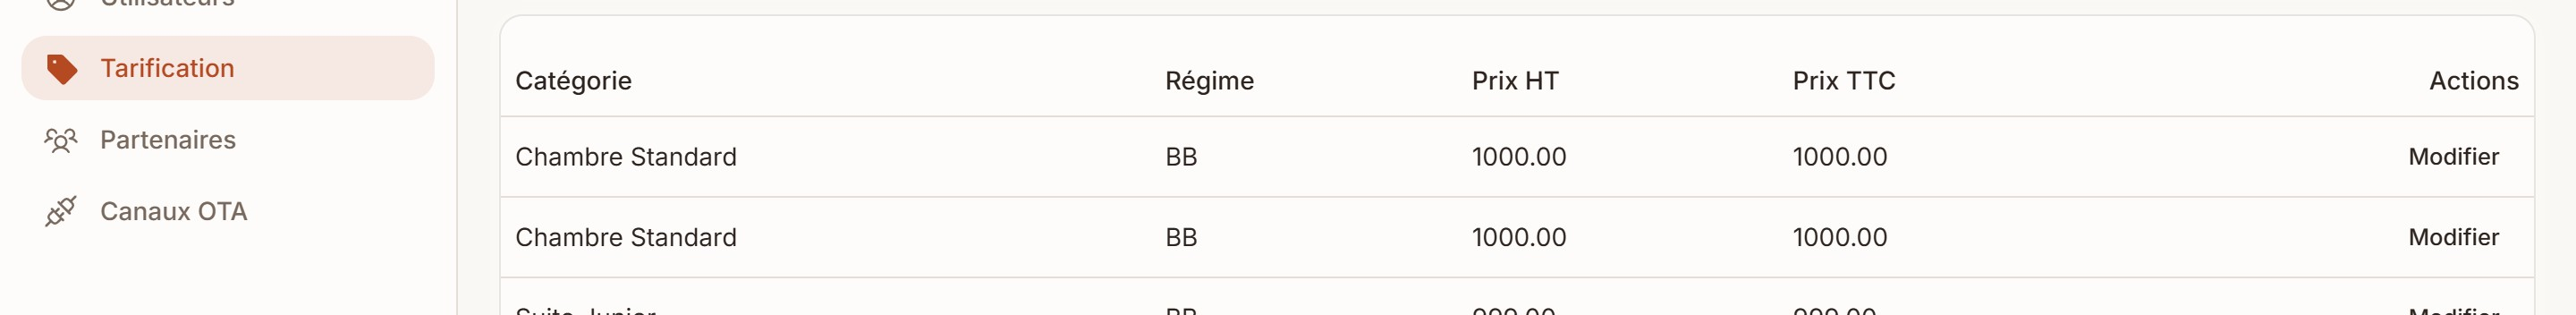
\includegraphics[width=0.85\textwidth]{figures/pic7_5as_ytzad_l_button_delete_.jpg}
\caption{Session de revue d'ergonomie et retours d'amélioration utilisateurs}
\label{fig:pic7}
\end{figure}

\section{Bilan des contributions individuelles de l'équipe}

Le Tableau~\ref{tab:contributions_detail} résume la répartition équilibrée des responsabilités et des réalisations au sein de notre trinôme d'élèves-ingénieurs.

\begin{table}[H]
\centering
\small
\renewcommand{\arraystretch}{1.3}
\begin{tabularx}{\textwidth}{|p{3.5cm}|X|}
\hline
\textbf{Élève-Ingénieur} & \textbf{Domaines de Responsabilité et Réalisations Majeures} \\
\hline
\textbf{Nabil BOUDARINE} & Architecture générale des 11 microservices, intégration et routage de la passerelle Kong API Gateway, sécurité Keycloak avec implémentation du standard WebAuthn/FIDO2 et flux QR Code, développement du moteur de clôture Night Audit transactionnel et archivage MinIO S3, conteneurisation globale sous Docker Compose. \\
\hline
\textbf{Youssef OUIZZA} & Conception et développement frontend sous Next.js 14 (App Router, Server Components, TypeScript, Tailwind CSS), implémentation du planning interactif Tape Chart avec glisser-déposer (\textit{Drag \& Drop}) et gestion des changements de chambre (\textit{Room Shift}), formulaires de réservation réactifs, intégration des WebSockets pour la synchronisation temps réel. \\
\hline
\textbf{Hamza IBN TALIB} & Développement des services de facturation et folios clients, implémentation des algorithmes de calcul fiscal marocain (TVA 10\%, TS 25 MAD, TPT 12 MAD), développement de l'application mobile progressive (PWA) Housekeeping pour le personnel d'étage, configuration du bus de messages RabbitMQ et rédaction des suites de tests unitaires automatisés sous Pytest. \\
\hline
\end{tabularx}
\caption{Répartition des contributions d'ingénierie au sein de l'équipe de projet}
\label{tab:contributions_detail}
\end{table}

\section{Difficultés techniques rencontrées et solutions d'ingénierie apportées}

Le Tableau~\ref{tab:defis_solutions} récapitule les principaux défis techniques surmontés durant les huit sprints de développement.

\begin{table}[H]
\centering
\small
\renewcommand{\arraystretch}{1.3}
\begin{tabularx}{\textwidth}{|p{3.5cm}|p{3.8cm}|X|}
\hline
\textbf{Défi Technique Rencontré} & \textbf{Cause Racine Identifiée} & \textbf{Solution d'Ingénierie Implémentée} \\
\hline
Collisions de réservations simultanées lors des tests de charge & Deux opérateurs sélectionnant la même chambre avant validation de la transaction SQL & Implémentation du pattern de verrouillage distribué Redis (\texttt{SET NX PX 10000}) avec bail temporel de 10 secondes et clé d'idempotence unique. \\
\hline
Lenteur excessive du Night Audit initial ($> 6$ minutes) & Boucle séquentielle bloquante sur chaque folio avec requêtes SQL unitaires & Parallélisation des calculs fiscaux par coroutines asynchrones (\texttt{asyncio.gather}) et requêtes d'insertion en masse (\textit{Batch SQL Inserts}), ramenant la durée à 45 secondes. \\
\hline
Pertes de messages AMQP lors du redémarrage d'un service & Files d'attente RabbitMQ configurées en mode volatile avec accusé de réception automatique & Configuration des files et échanges en mode durable (\textit{durable=True}) avec acquittement manuel (\textit{manual ack}) après confirmation de traitement. \\
\hline
Erreurs d'arrondis sur les montants de taxes marocaines & Utilisation du type flottant natif provoquant des dérives sur les centimes & Migration de l'ensemble des attributs financiers vers le type \texttt{Decimal} avec arrondi bancaire symétrique (\textit{ROUND\_HALF\_EVEN}). \\
\hline
Désynchronisation du Tape Chart lors de navigations multi-onglets & Connexion WebSocket fermée lors du passage en arrière-plan du navigateur & Implémentation de la \textit{BroadcastChannel API} permettant le partage de l'état d'occupation en temps réel entre tous les onglets du même navigateur. \\
\hline
\end{tabularx}
\caption{Synthèse des défis techniques et des solutions d'ingénierie apportées}
\label{tab:defis_solutions}
\end{table}

\section{Conclusion}

Ce quatrième chapitre a présenté la concrétisation intégrale de la plateforme logicielle \textbf{PMS AMH Hospitality}. À travers l'architecture technique microservices et la présentation illustrée de l'ensemble des 15 interfaces utilisateurs réelles développées, nous avons démontré l'adéquation de la solution aux contraintes opérationnelles du terrain hôtelier. Le chapitre suivant sera consacré à la stratégie d'assurance qualité, aux campagnes de tests et à l'évaluation de la qualité logicielle via SonarQube.
